\documentclass{report}

\input{~/dev/latex/template/preamble.tex}
\input{~/dev/latex/template/macros.tex}

\title{\Huge{}}
\author{\huge{Nathan Warner}}
\date{\huge{}}
\pagestyle{fancy}
\fancyhf{}
\lhead{Warner \thepage}
\rhead{}
% \lhead{\leftmark}
\cfoot{\thepage}
\setborder
% \usepackage[default]{sourcecodepro}
% \usepackage[T1]{fontenc}
\usepackage{pgfplots}
\pgfplotsset{compat=1.18}

\begin{document}
    % \maketitle
        \begin{titlepage}
       \begin{center}
           \vspace*{1cm}
    
           \textbf{Chapters 1-4}
    
           \vspace{0.5cm}
           Stat 128: Elementary Statistics
            
                
           \vspace{1.5cm}
   
           A Document By: \\
           \textbf{Nathan Warner}
    
           \vfill
                
                
           \vspace{0.8cm}
         
           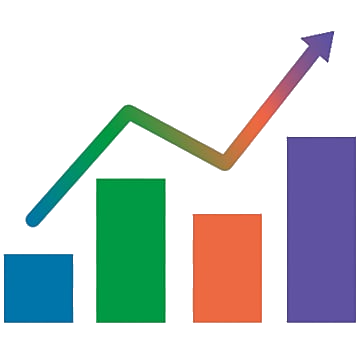
\includegraphics[width=0.4\textwidth]{./figures/2.png} \\
            July 03, 2023  \\
           Computer Science \\
           Joliet Junior College \\
           United States\\
           
                
       \end{center}
    \end{titlepage}
    \tableofcontents
    \pagebreak \bigbreak \noindent
    \section{Learning Outcomes}
    \bigbreak \noindent 
    \textbf{Chapter 1:}
    \begin{enumerate}
        \item Define data collection techniques including observational studies and design of experiments.
        \item Identify appropriate sampling methods.
    \end{enumerate}
    \bigbreak \noindent 
    \textbf{Chapter 2:}
    \begin{enumerate}
        \item Differentiate qualitative and quantitative data graphically. \\ This includes graphs such as bar plots, histograms, and dot plots.
    \end{enumerate}
    \bigbreak \noindent 
    \textbf{Chapter 3:}
    \begin{enumerate}
        \item Calculate measures of central tendency for data.
        \item Explain the concept of resistance.
        \item Decide which measure of central tendency to report for various data sets.
        \item Determine measures of dispersion for data.
        \item Determine standard scores, percentiles, and quartiles.
        \item Identify outliers using quartiles.
        \item Interpret boxplots.
    \end{enumerate}
    \bigbreak \noindent 
    \textbf{Chapter 4:}
    \begin{enumerate}
        \item Evaluate the linear correlation coefficient for bivariate quantitative data.
        \item Evaluate whether the coefficient is significant at a given level.
        \item Explain the difference between correlation and causation.
        \item Determine the least-squares regression equation for a given set of bivariate data.
        \item Predict values of the dependent variable using the least-squares regression equation.
        \item Interpret the slope and intercept of the least-squares regression equation.
        \item Test the requirements of the least-squares regression model using residual analysis.
        \item Determine and interpret the coefficient of determination.
        \item Graphically analyze bivariate quantitative data for outliers and influential observations.
        \item Describe the association between two qualitative variables using conditional distributions.
        \item Explain Simpson’s Paradox.
    \end{enumerate}

    \pagebreak \bigbreak \noindent
    \section{Chapter 1:}

    \bigbreak \noindent 
    \subsection{1.1: Introduction to the Practice of Statistics}

    \bigbreak \noindent 
    \textbf{\textit{\underline{Objectives for this section.}}}
    \begin{enumerate}
        \item Define Statistics and Statistical Thinking
        \item Explain the Process of Statistics
        \item Distinguish between Qualitative and Quantitative Variables
        \item Distinguish Between Discrete and Continuous Variables.
    \end{enumerate}
    
    \bigbreak \noindent \bigbreak \noindent 
    \textbf{\textit{\underline{Define Statistics and Statistical Thinking:}}}
    \bigbreak \noindent
        Statistics is the science of collecting, organizing, summarizing, and analyzing information to draw conclusions or answer questions. In addition, statistics is about providing a measure of confidence in any conclusions.
        \bigbreak \noindent 
        \textbf{Note:} We must report a measure of our confidence in our results because we do not have 100\% certainty our answers are correct.
        \bigbreak \noindent 
        The information referred to in the definition above is \textit{data}. \textbf{Data} are a "fact or proposition used to draw a conclusion or make a decision." Data describes characteristics of an individual.
        \bigbreak \noindent 
        One crucial thing to understand about \textbf{data}, is that is \textbf{varies}. One thing that makes an interesting study is the fact that the data within the study varies. A study about number of hearts a human has is not only uninteresting but not worth doing. This is because the data does not vary.
        \bigbreak \noindent 
        \textbf{Two Major Goals:}
        \begin{enumerate}
            \item Describe Variability.
            \item Understand sources of Variability.
        \end{enumerate}
        \bigbreak \noindent 
        In Statistics, the same approach to solving a problem can still lead to different results. This does not happen in a math class.
        \vspace{1em}

        \bigbreak \noindent \bigbreak \noindent 
        \textbf{\textit{\underline{Explain the Process of Statistics.}}}
        \bigbreak \noindent 
        First lets define some vocabulary:
        \begin{itemize}
            \item \textbf{Population:} The entire group to be studied is called the population.
            \item \textbf{Sample:} In statistics, it is often impractical or impossible to get access to the entire \textbf{population}, which is why we only look at a \textbf{sample.} A sample is a \textbf{subset} of the population being studied.
            \item \textbf{Individual:} An individual is a person or object that is a member of the population being studied.
            \item \textbf{Statistic:} A statistic is a numerical summary of a sample.
            \item \textbf{Descriptive Statistics:} Descriptive statistics consist of organizing and summarizing data. Descriptive statistics describe data through numerical summaries, tables, and graphs.
            \item \textbf{Inferential Statistics:} inferential Statistics uses methods that take a result from a sample, extend it to the population, and measure the reliability of the result.
            \item \textbf{Parameter:} A parameter is a numerical summary of a population.
        \end{itemize}

        \bigbreak \noindent 
        \textbf{The process of statistics:}
        \begin{enumerate}
            \item Identify the problem to be solved. It is important to clearly lay out the questions that the researcher wants answered, along with clearly specifying which population the study applies.
            \item Collect the data.
            \item Describe the data.
            \item Preform inference.
        \end{enumerate}

        \bigbreak \noindent 
        \begin{mdframed}
          \textbf{Example: The AP - National Constitution Center conducted a national poll to learn how adult Americans feel existing gun-control laws infringe on the second amendment to the U.S Constitution}
          \bigbreak \noindent 
          \textbf{The Following statistical process allowed the researchers to conduct their study.}
          \begin{enumerate}
              \item \textbf{Identify the research objective.}: The researchers wished to determine the percentage of adult Americans who believe gun-control laws infringe on the public's right to bear arms.
            \item \textbf{Collect the information needed to answer the question posed in (1).}: It is unreasonable to expect to survey the more than 200 million adult Americans to determine how they feel about gun-control laws. So the researchers surveyed a sample of 1007 adult Americans. Of those surveyed, 514 stated they believe existing gun-control laws infringe on the public's right to bear arms.
            \item \textbf{Describe the data.}: Of the 1007 individuals in the survey, 51\% believe existing gun-control laws inferring on the public's right to bear arms. This is a descriptive statistic, because its value is determined from a sample.
            \item \textbf{Preform inference.}: The researchers at the AP - National Constitution Center wanted to extend the results of the survey to \textbf{all} adult Americans. When generalizing results from a sample to a population, the results are \textbf{uncertain}. To account for this uncertainty, researchers reported a 3\% \textit{margin of error.} This means that the researchers feel fairly certain (in fact, 95\% certain) that the percentage of \textit{all} adult Americans who believe existing gun-control laws infringe on the public's right to bear arms is somewhere between 48\% and 54\%

          \end{enumerate}
          
        \end{mdframed}

        \bigbreak \noindent \bigbreak \noindent 
        \textbf{\textit{\underline{Distinguish between Qualitative and Quantitative Variables}}}
        \bigbreak \noindent 
        First let's define some vocab:
        \begin{itemize}
            \item \textbf{Variables:} The characteristics of the individuals in a study. Variables vary, which means they can take on different values.
            \item \textbf{Constants:} Variables that do not vary. Inferential statistics is not necessary with constants.
        \end{itemize}
        \bigbreak \noindent 
        One goal of research is to learn the causes of variability.
        \bigbreak \noindent 
        Variables can be classified into two groups: qualitative and quantitative.
        \begin{itemize}
            \item \textbf{Qualitative, or categorical variables} allow for the classification of individuals base on some attribute or characteristic.
            \item \textbf{Quantitative variables} provide numerical measures of individuals. The values of a quantitative variable can be added or subtracted and provide meaningful results.
        \end{itemize}
        \bigbreak \noindent 
        \begin{mdframed}
          \textbf{Example: Determine whether the following variables are qualitative or quantitative.}
          \begin{enumerate}[label=\alph*.)]
              \item \textbf{Gender.}: Qualitative
              \item \textbf{Temperature.}: Quantitative
              \item \textbf{Number of days during the past week that a college student studied.}: Quantitative
              \item \textbf{Zip Code.} Qualitative
          \end{enumerate}
          \textbf{Caution:} A numeric value does not automatically suggest a variable is quantitative.
        \end{mdframed}

        \bigbreak \noindent 
        \textbf{\textit{\underline{Distinguish between Discrete and Continuous Variables.}}}
        \begin{itemize}
            \item A \textbf{discrete variable} is a quantitative variable that has either a finite number of possible values or a countable number of possible values. A discrete variable cannot take on every possible value between any two possible values.
            \item A \textbf{continuous variable} is a quantitative variable that has an infinite number of possible values that are not countable. A continuous variable may take on every possible value between any two values. Continuous variables typically result from measurement. Continuous variables are often rounded. If a certain make of car gets 24 miles per gallon (mpg) of gasoline, its miles per gallon must be greater than or equal to 23.5 and less than 24.5, or $23.5 \leq mpg \leq 24.5$
        \end{itemize}

        \bigbreak \noindent 
        This Figure illustrates the relationship among qualitative, quantitative, discrete, and continuous variables.

        \begin{figure}[ht]
            \centering
            \incfig{graph1}
            \label{fig:graph1}
        \end{figure}

        \bigbreak \noindent 
        \begin{mdframed}
          \textbf{Example: Distinguish whether the quantitative variables are discrete or continuous.}
          \begin{enumerate}[label=\alph*.)]
            \item \textbf{The number of heads obtained after flipping a coin five times.}: Discrete
            \item \textbf{The number of cars that arrive at a McDonald's drive through between 12:00 PM and 1:00 PM}: Discrete
            \item \textbf{The Distance a 2011 Toyota Prius can travel in city driving conditions with a full tank of gas.}: Continuous
          \end{enumerate}
        \end{mdframed}

        \bigbreak \noindent 
        \textbf{Vocab:}
        \begin{itemize}
            \item The list of observed values for a variable is \textbf{data.}
            \item \textbf{Qualitative data} are observations corresponding to a \textbf{qualitative variable.}
            \item \textbf{Quantitative data} are observations corresponding to a quantitative variable.
            \item \textbf{Discrete data} are observations corresponding to a discrete variable.
            \item \textbf{Continuous data} are observations corresponding to a continuous variable.
        \end{itemize}

        \bigbreak \noindent 
        \begin{mdframed}
          \textbf{Example: Distinguish between Variables and Data}
          \bigbreak \noindent 
          The following table presents a group of selected countries and information regarding these countries.
          \bigbreak \noindent 
          Identify the individuals, variables, and data.
          \begin{center}
              \begin{tabular}{|l|c|c|c|}
              \hline
              Country & Government Type & Life Expectancy (Years) & Population (in millions) \\
              	\hline
              Australia & Federal parliamentary democracy & 81.63 & 21.3   \\
              	\hline
            Canada & Constitutional monarchy & 81.23 & 33.5 \\
            \hline
            France & Republic & 80.98 & 64.4 \\
            \hline
            Morocco & Constitutional monarchy & 75.47 & 31.3 \\
            \hline
            Poland & Republic & 75.63 & 38.5 \\
            \hline
            Sri Lanka & Republic & 75.14 & 21.3\\
            \hline
            United States & Federal Republic & 78.11 & 307.2 \\
            \hline
              \end{tabular}
          \end{center}
          \bigbreak \noindent 
          \textbf{Qualitative}: Government Type \\
          \textbf{Quantitative}: Life Expectancy and Population \\
          \textbf{Continuous}: Life Expectancy \\
          \textbf{Discrete}: Population \\
          \textbf{Data}: Everything under Government Type, Life Expectancy, and Population.
      \item 
        \end{mdframed}

        \pagebreak \bigbreak \noindent
        \begin{center}
            \begin{large}
                \textbf{All Vocab / Concepts From Section 1.1}
            \end{large}
        \end{center}
        \line(1,0){490}
        \begin{itemize}
            \item \textbf{Population:} The entire group to be studied is called the population.
            \item \textbf{Sample:} In statistics, it is often impractical or impossible to get access to the entire \textbf{population}, which is why we only look at a \textbf{sample.} A sample is a \textbf{subset} of the population being studied.
            \item \textbf{Individual:} An individual is a person or object that is a member of the population being studied.
            \item \textbf{Statistic:} A statistic is a numerical summary of a sample.
            \item \textbf{Descriptive Statistics:} Descriptive statistics consist of organizing and summarizing data. Descriptive statistics describe data through numerical summaries, tables, and graphs.
            \item \textbf{Inferential Statistics:} inferential Statistics uses methods that take a result from a sample, extend it to the population, and measure the reliability of the result.
            \item \textbf{Parameter:} A parameter is a numerical summary of a population.
            \item \textbf{Variables:} The characteristics of the individuals in a study. Variables vary, which means they can take on different values.
            \item \textbf{Constants:} Variables that do not vary. Inferential statistics is not necessary with constants.
            \item \textbf{Data:} The list of observed values for a variable.
            \item \textbf{Qualitative data} are observations corresponding to a \textbf{qualitative variable.}
            \item \textbf{Quantitative data} are observations corresponding to a quantitative variable.
            \item \textbf{Discrete data} are observations corresponding to a discrete variable.
            \item \textbf{Continuous data} are observations corresponding to a continuous variable.
        \end{itemize}

        \bigbreak \noindent 
        \textbf{Concepts:}
        \begin{itemize}
            \item Statistics and Statistical Thinking.
            \item Describe Variability
            \item Understand Sources of variability
            \item Statistical studies are concerned with both describing the variability in the data and understanding the sources of variability in data. Understanding the sources allows researchers to control it and reach better conclusions.
            \item The process of statistics
            \item Inferential/Descriptive Statistics
            \item Variables
                \begin{itemize}
                    \item Qualitative (Categorical) / Quantitative
                    \item Discrete / Continuous
                \end{itemize}
            \item Data
                \begin{itemize}
                    \item Qualitative (Categorical) / Quantitative
                    \item Discrete / Continuous
                \end{itemize}
        \end{itemize}

        \pagebreak \bigbreak \noindent
        \subsection{1.2: Observational Studies versus Designed Experiments}
        \bigbreak \noindent 
        \textbf{\textit{\underline{Objectives for this section.}}}
        \begin{enumerate}
            \item Distinguish between an Observational Study and a Designed Experiment
            \item Explain the Various Types of Observational Studies
        \end{enumerate}

        \bigbreak \noindent 
        \textbf{\textit{\underline{Distinguish between an Observational Study and a Designed Experiment}}}
        \begin{itemize}
            \item \textbf{Observational studies:} Observational studies involve observing and analyzing data collected from real-world settings without any intervention or manipulation by the researcher. Researchers passively observe and record information to identify correlations or associations between variables.
            \item \textbf{Designed experiments:} Designed experiments, also known as randomized controlled trials (RCTs), involve researchers actively manipulating variables and randomly assigning participants to different groups. This allows researchers to establish cause-and-effect relationships by comparing the effects of different interventions or treatments on the outcome of interest.
        \end{itemize}
        \bigbreak \noindent 
        \textbf{Vocab:}
        \begin{itemize}
            \item \textbf{Explanatory Variable:} An explanatory variable, also known as an independent variable or predictor variable, is a variable that is manipulated or controlled by researchers in an experiment or study. It is the variable that is hypothesized to have an impact on the outcome or dependent variable. 
            \item \textbf{Lurking variable}: An explanatory variable that was not considered in a study, but that affects the value of the response variable.
            \item \textbf{Response Variable}: The response variable, also known as the dependent variable or outcome variable, is the variable that is measured or observed to determine the effect or response of the explanatory variable(s). It is the variable that researchers are interested in studying or predicting. 
            \item \textbf{Confounding:} Occurs when the effects of two or more explanatory variables are not separated. Therefore, any relation that may exist between an explanatory variable and the response variable may be due to some other variable or variables not accounted for in the study.
            \item \textbf{Census:} List of individuals in a population along with certain characteristics of each individual.
        \end{itemize}

        \bigbreak \noindent 
        \nt{Is observational studies, we \textbf{are not} allowed to make statements of \textit{causality}, meaning we cannot say that changes in the explanatory variable \textit{cause} changes in the response variable. We can only say changes in the explanatory variable are associated with changes in the response variable.}

        \bigbreak \noindent 
        Why would we ever conduct an observational study if we cannot claim causation? Because it is often unethical to conduct a designed experiment.
        \bigbreak \noindent 
        Consider the link between smoking and lung cancer. In a designed experiment (on humans) to determine if smoking causes lung cancer, a researcher would divide a group of volunteers into two groups—Group 1 would smoke a pack of cigarettes every day for the next 10 years, and Group 2 would not smoke. Eating habits, sleeping habits, and exercise would be controlled so that the only difference between the two groups would be smoking. After 10 years, the experiment's researcher would compare the proportion of participants in the study who contract lung cancer in the smoking group with the nonsmoking group. If the two proportions differ significantly, it could be said that smoking causes lung cancer. This designed experiment controls many potential cancer-causing factors that would not be controlled in an observational study. However, it is an unethical experiment. Do you see why?
        \bigbreak \noindent Other reasons exist for conducting observational studies over designed experiments. An article in support of observational studies states, "Observational studies have several advantages over designed experiments, including lower cost, greater timeliness, and a broader range of patients." From Kjell Benson, BA, and Arthur J. Hartz, MD, PhD. "A Comparison of Observational Studies and Randomized Controlled Trials." 

        \bigbreak \noindent 
        In designed experiments, it is possible to have two explanatory variables in a study that are related to each other and related to the response variable. For example, suppose Professor Egner wanted to conduct an experiment in which she compared student success using online homework versus traditional textbook homework. To do the study, she taught her morning statistics class using the online homework and her afternoon class using traditional textbook homework. At the end of the semester, she compared the final exam scores for the online section to the textbook section. If the morning section had higher scores, could Professor Egner conclude that online homework is the cause of higher exam scores? Not necessarily. It is possible that the morning class had students who were more motivated. It is impossible to know whether the outcome was due to the online homework or to the time at which the class was taught. In this sense, we say that the time of day the class is taught is a confounding variable.

        \bigbreak \noindent 
        \textbf{Lurking Vs Confounding Variables:}
        \bigbreak \noindent 
        The big difference between lurking variables and confounding variables is that lurking variables are not considered in the study (for example, we did not consider lifestyle in the pneumonia study) whereas confounding variables are measured in the study (for example, we measured morning versus afternoon classes).
        \bigbreak \noindent 
        So lurking variables are related to both the explanatory and response variables, and this relation is what creates the apparent association between the explanatory variable and response variable in the study. For example, lifestyle (healthy or not) is associated with the likelihood of getting an influenza shot as well as the likelihood of contracting pneumonia or influenza.
        \bigbreak \noindent 
        A confounding variable is a variable in a study that does not necessarily have any association with the other explanatory variable but does have an effect on the response variable. Perhaps morning students are more motivated, and this is what led to the higher final exam scores, not the homework delivery system.
        \bigbreak \noindent 
        The bottom line is that both lurking variables and confounding variables can confound the results of a study, so a researcher should be mindful of their potential existence.

        \bigbreak \noindent \bigbreak \noindent 
        \textbf{\textit{\underline{Explain the Various Types of Observational Studies}}}
        \bigbreak \noindent 
        \begin{itemize}
            \item \textbf{Cross-sectional Studies:} Observational studies that collect information about individuals at a specific point in time, or over a very short period of time.
            \item \textbf{case-control Studies:} These studies are \textbf{retrospective,} meaning that they require individuals to look back in time or require the researcher to look at existing records. In case-control studies, individuals that have certain characteristics are matched with those that do not.
                \begin{itemize}
                    \item \textbf{Positive:} Control group allows for a comparison
                    \item \textbf{Negative:} Individuals must remember details
                    \item \textbf{Negative:} Records might not exist
                \end{itemize}
            \item \textbf{Cohort Studies:} A cohort study first identifies a group of individuals to participate in the study (cohort). The cohort is then observed over a period of time. Over this time period, characteristics about the individuals are recorded. Because the data is collected over time, cohort studies are \textbf{prospective.}
                \begin{itemize}
                    \item \textbf{Advantage:} Researcher does not need to rely on memory of study participants or existing records.
                    \item \textbf{Disadvantage:} Requires a lot of time.
                    \item \textbf{Disadvantage:} Could be expensive.
                \end{itemize}
        \end{itemize}

        \pagebreak \bigbreak \noindent
        \textbf{Is a designed experiment superior to an observational study? Not necessarily.}
        \begin{itemize}
            \item Because cross-sectional and case-control observational studies are relatively inexpensive, they allow researchers to explore possible associations prior to undertaking large cohort studies or designed experiments.
            \item It is not always possible to conduct an experiment. For example, we could not conduct an experiment to investigate the perceived link between high-tension wires and leukemia (on humans). Do you see why?
        \end{itemize}

        \pagebreak \bigbreak \noindent
        \subsection{1.3: Simple Random Sampling}
        \bigbreak \noindent 
        \textbf{\textit{\underline{Learning Objectives for this section.}}}
        \begin{enumerate}
            \item Obtain a simple random sample
        \end{enumerate}
        \bigbreak \noindent 
        \textbf{Vocab:}
        \begin{itemize}
            \item \textbf{Random Sampling:} The process of using chance to select individuals from a population to be included in the sample.
            \item \textbf{Simple Random Sampling:} A sample of size $n$  from a population of size $N $  is obtained through simple random sampling if every possible sample of size $n$  has an equal chance of occurring. The sample is then called a simple random sample.
                \begin{itemize}
                    \item $n < N $
                \end{itemize}
            \item \textbf{frame:} a list of all the individuals within the population.
            \item \textbf{Sample Without Replacement:} Once an individual is selected, the individual cannot be selected again.
        \end{itemize}

        \bigbreak \noindent 
        \nt{For the results of a survey to be reliable, the characteristics of the individuals in the sample must be representative of the characteristics of the individuals in the population. The key to obtaining a sample representative of a population is to let chance or randomness, rather than convenience, play a role in dictating which individuals are in the sample. If convenience is used to obtain a sample, the results of the survey are meaningless.}

        \bigbreak \noindent 
        \textbf{Recognizing a Convenience Sample and Its Limitations:}
        \bigbreak \noindent 
        Suppose that Gallup wants to know the proportion of adult Americans who consider themselves to be baseball fans. If Gallup obtained a sample by standing outside Fenway Park (home of the Boston Red Sox professional baseball team), the survey results are not likely to be reliable. Why? Clearly, the individuals in the sample do not accurately reflect the makeup of the entire population.
        \bigbreak \noindent 
        Suppose you wanted to learn the proportion of students on your campus who work. It might be convenient to survey the students in your statistics class, but do these students represent the overall student body? Does the proportion of freshmen, sophomores, juniors, and seniors in your class mirror the proportion of freshmen, sophomores, juniors, and seniors on campus? Does the proportion of males and females in your class resemble the proportion of males and females across campus? Probably not. What about evening (or day) students? For these (and many other) reasons, the convenient sample is not representative of the population, which means that any results reported from your survey are misleading.

        \bigbreak \noindent 
        \textbf{Effective Sampling Techniques:}
        \begin{enumerate}
            \item \textbf{Simple random sampling}
            \item \textbf{Stratified sampling}
            \item \textbf{Systematic sampling}
            \item \textbf{Cluster sampling}
        \end{enumerate}
        \bigbreak \noindent 
        These sampling methods are designed so that any selection biases the surveyor introduced (knowingly or unknowingly) during the selection process are eliminated. In other words, the surveyor does not have a choice as to which individuals are in the study. We will discuss simple random sampling in this section and the remaining three types of sampling in the next section.

        \bigbreak \noindent 
        \begin{mdframed}
          \textbf{Bonus: Consider a set of 5 possibilities A-E, and we want to determine the total number of combinations of selecting 3 letters:}
          \bigbreak \noindent 
          We can use the formula:
          \begin{align*}
              nCk = \frac{n!}{(k!(n-k)!)}
          .\end{align*}
          \bigbreak \noindent 
          Where $n $ is the total number of classes in the course list and $k$ is the number of classes to be chosen.
          \bigbreak \noindent 
          So we have $n =5$ and $k = 3$:
          \begin{align*}
                \frac{5!}{(3!(5-3)!)} \\
                = \frac{5!}{3! \cdot 2!}\\
                 = \frac{5 \cdot 4 \cdot 3!}{3! \cdot 2\cdot 1} \\
                 = \frac{5 \cdot 4}{2\cdot 1} \\
                 = \frac{20}{2} \\
                 = 10
          .\end{align*}
          \bigbreak \noindent 
          And we can calculate the chance over a certain event happening with:
          \begin{align*}
              Probablility = \frac{Number of Occurences}{Total Number of Occurences}
          .\end{align*}
        \end{mdframed}

        \bigbreak \noindent 
        \textbf{How do we select the individuals in a simple random sample?}
        \bigbreak \noindent 
        We could write the names of the individuals in the population on different pieces of paper and then select names from a hat. Often, however, the size of the population is so large that performing simple random sampling in this fashion is not practical.
        \bigbreak \noindent 
        Typically, each individual in the population is assigned a unique number between 1 and $N$, Where $N$ is the size of the population. Then $n $ distinct random numbers are selected, where $n $ is the size of the population
        \bigbreak \noindent 
        To number the individuals in the population, we need a \textbf{frame:} a list of all the individuals within the population.

        \bigbreak \noindent 
        \textbf{Obtaining a simple random sample with calculator (ti-84)}
        \bigbreak \noindent 
        The accounting firm of Senese and Associates has grown. To make sure their clients are still satisfied with the services they are receiving, the company decides to send a survey out to a simple random sample of 5 of its 30 clients.
        \bigbreak \noindent 
        So we need 5 unique random numbers from a range of 1-30. To do this in our ti-84 calculator:
        \begin{enumerate}
            \item Math $\rightarrow$ Prod $\rightarrow$ randIntNorep
            \item Syntax: randIntNoRep(\textit{lowerbound}, \textit{upperbound}, \textit{$n$}), where $n$ is the number of unique random numbers we must generate.
            \item Lower: 1
            \item Upper: 30
            \item $n$: 5
            \item Select Paste.
        \end{enumerate}

        \pagebreak \bigbreak \noindent
        \subsection{1.4: Other Effective Sampling Methods}
        \bigbreak \noindent 
        \textbf{\textit{\underline{Learning Objectives For This Section.}}}
        \begin{enumerate}
            \item \textbf{Obtain a Stratified Sample}
            \item \textbf{Obtain a Systematic Sample}
            \item \textbf{Obtain a Cluster Sample}
        \end{enumerate}
        \bigbreak \noindent 
        \textbf{Vocab:}
        \begin{itemize}
            \item \textbf{Stratified sample}: is obtained by dividing the population into nonoverlapping groups called strata and then obtaining a simple random sample from each stratum. The individuals within each stratum should be homogenous (similar) in some way.
                \begin{itemize}
                    \item Within Stratified samples, the number of individuals sampled from each stratum should be proportional to the size of the strata in the population.
                \end{itemize}
            \item \textbf{Systematic sample} is obtained by selecting every $k$th individual from the population. The first individual selected corresponds to a number between 1 and $k$
            \item \textbf{Cluster sample} is obtained by selecting all individuals within a randomly selected collection or group of individuals.
            \item \textbf{Convenience sample:} the individuals are easily obtained and not based on randomness.
        \end{itemize}
        \bigbreak \noindent 
        \textbf{\textit{\underline{Obtaining a Stratified Sample:}}}
        \bigbreak \noindent 
        Suppose Congress was considering a bill that abolishes estate taxes. In an effort to determine the opinion of her constituency, a senator asks a pollster to conduct a survey within her state.
        \bigbreak \noindent 
        The pollster may divide the population of registered voters within the state into three strata: Republican, Democrat, and Independent. This grouping makes sense because the members within each of the three parties may have similar opinions regarding estate taxes, but opinions among parties may differ. The main criterion in performing a stratified sample is that each group (stratum) must have a common attribute that results in the individuals being similar within the stratum.
        \bigbreak \noindent 
        An advantage of stratified sampling over simple random sampling is that it may allow fewer individuals to be surveyed while it obtains the same or more information. This result occurs because individuals within each subgroup have similar characteristics, so opinions within the group are not as likely to vary much from one individual to the next. In addition, a stratified sample guarantees that each stratum is represented in the sample.

        \bigbreak \noindent \bigbreak \noindent 
        \textbf{\textit{\underline{Obtaining a Systematic Sample:}}}
        \bigbreak \noindent 
        For example, to learn about the outcome of an election, a pollster might survey every tenth individual that leaves a polling place.
        \bigbreak \noindent 
        Because systematic sampling does not require a frame, it is a useful technique when you cannot gather a list of the individuals in the population. Also, systematic samples typically provide more information for a given cost than does simple random sampling. In addition, systematic sampling is easier to employ; so there is less likelihood of interviewer error occurring, such as selecting the wrong individual to be surveyed.

        \bigbreak \noindent 
        \textbf{Choosing a value for $k $}:
        \bigbreak \noindent 
        If the size of the population is unknown, there is no mathematical way to determine $k$
        \bigbreak \noindent 
        The value  of $k$ must be small enough to achieve our desired sample size.
        \bigbreak \noindent 
        The value of $k$ must be large enough to obtain a sample that is representative of the population.

        \bigbreak \noindent 
        \begin{mdframed}
            \textbf{Example:}
            Suppose we have a scenario where $k = 30$, and we want to start with individual 3 and select 40 individuals.
            \bigbreak \noindent 
            Firstly, we can observe that the sequence follows an arithmetic progression.
            \bigbreak \noindent 
            We can represent the sequence as:
            \bigbreak \noindent 
            \[a_{40} = \{3, 33, 63, \ldots, a_{40}\}\]
            \bigbreak \noindent 
            To find the 40th term, $a_{40}$, we can use the formula:
            \bigbreak \noindent 
            \[a_{n} = a + (n-1)d,\quad \text{where } n = 40,\ d = 30\]
            \bigbreak \noindent 
            Substituting the values into the formula:
            \bigbreak \noindent 
            \[a_{40} = 3 + (40-1) \cdot 30 = 1173\]
            \bigbreak \noindent 
            Therefore, our sequence is:
            \bigbreak \noindent 
            \[a_{40} = \{3, 33, 63, \ldots, 1173\}\]
            \bigbreak \noindent 
            \textbf{Note:} It's important to note that if our population does not have 1173 individuals, the desired sample size will not be achieved.
            \bigbreak \noindent 
        \end{mdframed}
        \bigbreak \noindent 
        \begin{mdframed}
          \textbf{Example: Now Suppose $k=4$}
          \bigbreak \noindent 
          \begin{align*}
              a_{40} = 3 + (40-1)\cdot 4 \\
              = 159
          .\end{align*}
          \bigbreak \noindent 
          So we have the sequence:
          \begin{align*}
              a_{40} = \{3,7,11,...,159\}
          .\end{align*}
          \bigbreak \noindent 
          \textbf{Note:} Suppose our population is Kroger shoppers, The $159^{th}$ shopper might leave the store at 3pm, so our survey would not include any of the evening shoppers.
        \end{mdframed}
        \bigbreak \noindent 
        \nt{An estimate of the size of the population would help to determine an appropriate value of $k $}

        \pagebreak \bigbreak \noindent
        \textbf{Systematic Sampling Determining $k$ when $N$ is Known:}
        \bigbreak \noindent 
        Steps to deduce $k$:
        \begin{enumerate}
            \item If possible, approximate the population size $N$. 
            \item Determine the sample size desired, $n$. 
            \item Divide $N$ by $n$ \bigg($\frac{N}{n},$\bigg) and round down to the nearest integer. This value is $k$.
            \item Randomly select a number between $1\ and\ k$, call this number $a$ (starting point)
            \item The sample will consist of the following individuals:
                \begin{align*}
                    a_{n} = a, a + k, a +2k,..., a + (n-1)k
                .\end{align*}
        \end{enumerate}
        \bigbreak \noindent 
        \begin{mdframed}
          \textbf{Example: Suppose $N=20,325$ and we desire a sample size of $n=100$. }
          \bigbreak \noindent 
          \begin{align*}
              K= \frac{20,325}{100} \\
              K= 203
          .\end{align*}
          \bigbreak \noindent 
          Now let's further suppose that we start with the $90^{th}$ individual. 
          \bigbreak \noindent 
          To compute our arithmetic sequence with these parameters, first lets find $a_{100}$:
          \begin{align*}
              a_{100} = 90 + (100-1)\cdot 203 \\
              a_{100} = 19890
          .\end{align*}
          \bigbreak \noindent 
          So we have the sequence:
          \begin{align*}
              a_{100} = \{90, 293, 496,...,20187\}
          .\end{align*}
        \end{mdframed}

        \pagebreak \bigbreak \noindent
        \textbf{\textit{\underline{Obtain a Cluster Sample.}}}
        \bigbreak \noindent 
        Suppose a school administrator wants to learn the characteristics of students enrolled in online classes. Rather than obtaining a simple random sample based on the frame of all students enrolled in online classes, the administrator treats each online class as a cluster and then finds a simple random sample of these clusters. The administrator then surveys all students in the selected clusters. This reduces the number of classes that get surveyed.
        \bigbreak \noindent 
        The following questions arise in cluster sampling:
        \begin{itemize}
            \item How do I cluster the population?
            \item How many clusters do I sample?
            \item How many individuals should be in each cluster?
        \end{itemize}
        \bigbreak \noindent 
        First, we must determine whether the individuals within the proposed cluster are homogeneous or heterogeneous.
        \bigbreak \noindent 
        city blocks tend to have similar households. Survey responses from houses on the same city block are likely to be similar. This results in duplicate information. We conclude that if the clusters have homogeneous individuals, it is better to have more clusters with fewer individuals in each cluster.
        \bigbreak \noindent 
        What if the cluster is heterogeneous? Under this circumstance, the heterogeneity of the cluster likely resembles the heterogeneity of the population. In other words, each cluster is a scaled-down representation of the overall population.
        \bigbreak \noindent 
        For example, a quality control manager might use shipping boxes that contain 100 light bulbs as a cluster. The manager does this because the rate of defects within the cluster resembles the rate of defects in the population, assuming that the bulbs are randomly placed in the box. Thus, when each cluster is heterogeneous, fewer clusters with more individuals in each cluster are appropriate.

        \bigbreak \noindent 
        \textbf{Convenience Sampling:}
        \bigbreak \noindent 
        In the four sampling techniques just presented (simple random sampling, stratified sampling, systematic sampling, and cluster sampling), the individuals are selected randomly. Often, however, inappropriate sampling methods are used in which the individuals are not randomly selected.
        \bigbreak \noindent 
        Have you ever been stopped in the mall by someone holding a clipboard? These folks are responsible for gathering information, but their methods of data collection are inappropriate, and the results of their analysis are suspect because they collect data using a convenience sample.
        \bigbreak \noindent 
        The most popular convenience samples are those in which the individuals in the sample are self-selected, meaning the individuals themselves decide to participate in the survey. Self-selected surveys are also called voluntary response samples. One example of self-selected sampling is phone-in polling—a radio personality will ask his or her listeners to phone or text the station to submit their opinions. Another example is the use of the Internet to conduct surveys. For example, a TV news show will present a story regarding a certain topic and ask its viewers to "tell us what you think" by completing an online questionnaire or tweeting an opinion with a hashtag.
        \bigbreak \noindent 
        Both of these samples are poor designs because the individuals who decide to be in the sample generally have strong opinions about the topic. A more typical individual in the population will not bother phoning, texting, or tweeting to complete a survey. Any inference made regarding the population from this type of sample should be made with extreme caution.

        \pagebreak \bigbreak \noindent
        \textbf{Multistage Sampling}
        \bigbreak \noindent 
        In practice, most large-scale surveys obtain samples using a combination of the techniques just presented.
        \bigbreak \noindent 
        As an example of multistage sampling, consider Nielsen Media Research. Nielsen randomly selects households and, through a People Meter, monitors the television programs these households are watching. The meter is an electronic box connected to each TV within the household. The People Meter measures what program is being watched and who is watching it. Nielsen selects the households with the use of a two-stage sampling process.
        \begin{enumerate}
            \item U.S. Census data, Nielsen divides the country into geographic areas (strata). The strata are typically city blocks in urban areas and geographic regions in rural areas. About 
            \item sends representatives to the selected strata and lists households within the strata. The households are then randomly selected through a simple random sample.
        \end{enumerate}
        Nielsen sells the information obtained to television stations and companies. These results are used to help determine prices for commercials.

        \bigbreak \noindent 
        \textbf{Sample Size Considerations:}
        \bigbreak \noindent 
        Throughout our discussion of sampling, we did not mention how to determine the sample size. Researchers need to know how many individuals they must survey to draw conclusions about the population within some predetermined margin of error.
        \bigbreak \noindent 
        Researchers must find a balance between the reliability of the results and the cost of obtaining these results. Time and money determine the level of confidence researchers will place on the conclusions drawn from the sample data. The more time and money researchers have available, the more accurate the results of the statistical inference will be.
        \bigbreak \noindent 
        Later in the course, we will discuss techniques for determining the sample size required to estimate characteristics regarding the population within some margin of error. (For a detailed discussion of sample size considerations, consult a text on sampling techniques such as Elements of Sampling Theory and Methods by Z. Govindarajulu, Pearson, 1999.)

        \pagebreak \bigbreak \noindent
        \subsection{1.5: Bias in Sampling}
        \bigbreak \noindent 
        \textbf{\textit{\underline{Learning Objectives For This Section:}}}
        \begin{enumerate}
            \item \textbf{Explain the Sources of Bias in Sampling}
        \end{enumerate}
        \bigbreak \noindent 
        \textbf{Vocab:}
        \begin{itemize}
            \item \textbf{Bias:} If the results of the sample are not representative of the population. Sampling bias means that the technique used to obtain the sample's individuals tends to favor one part of the  population over another. Any convenience sample has sampling bias because the individuals are not chosen through a random sample.
            \item \textbf{Undercoverage:} Occurs when the proportion of one segment of the population is lower in a sample than it is in the population. This can result if the frame used to obtain the sample is incomplete or not representative of the population.
            \item \textbf{Sampling bias:} sampling bias is a bias in which a sample is collected in such a way that some members of the intended population have a lower or higher sampling probability than others. It results in a biased sample of a population in which all individuals, or instances, were not equally likely to have been selected
            \item \textbf{Nonresponse bias:} exists when individuals selected to be in the sample who do not respond to the survey have different opinions from those who do
                \begin{itemize}
                    \item This can be controlled with \textbf{callbacks}.
                    \item This can also be controlled with \textbf{rewards or incentives}
                \end{itemize}
            \item \textbf{Response bias:} Exists when the answers on a survey do not reflect the true feelings of the respondent.
            \item \textbf{Open Question:} Allows the respondent to choose his or her response
            \item \textbf{Closed Question:} requires the respondent to choose from a list of predetermined responses
            \item \textbf{Nonsampling errors:} result from undercoverage, nonresponse bias, response bias, or data-entry error. Such errors could also be present in a census.
            \item \textbf{Sampling error:} results from using a sample to estimate information about a population. This type of error occurs because a sample gives incomplete information about a population.
        \end{itemize}
        \bigbreak \noindent 
        \textbf{\textit{\underline{Explain the sources of Bias in Sampling:}}}
        \bigbreak \noindent 
        There are three sources of bias in sampling:
        \begin{itemize}
            \item \textbf{Sampling bias}
            \item \textbf{Nonresponse bias}
            \item \textbf{Response bias}
        \end{itemize}
        \bigbreak \noindent 
        \textbf{Interviewer Error.}
        \bigbreak \noindent 
        Do not be quick to trust surveys conducted by poorly trained interviewers. 
        \bigbreak \noindent 
        Do not trust survey results if the sponsor has a vested interest in the results of the survey.
        \bigbreak \noindent 
        \textbf{Misrepresented Errors}
        \bigbreak \noindent 
        Some survey questions result in responses that misrepresent facts or are flat-out lies.
        \bigbreak \noindent 
        \textbf{Wording of Questions.}
        \bigbreak \noindent 
        The way a question is worded can lead to response bias in a survey, so questions must always be asked in balanced form.

        \bigbreak \noindent 
        \textbf{Ordering of Questions or Words}
        \bigbreak \noindent 
        Many surveys will rearrange the order of the questions within a questionnaire so that responses are not affected by prior questions.
        \bigbreak \noindent 
        \textbf{Type of Question.}
        \bigbreak \noindent 
        One of the first considerations in designing a question is determining whether the question should be \textit{open} or \textit{closed}
        \bigbreak \noindent 
        In closed questions, the possible responses should be rearranged because respondents are likely to choose early choices in a list rather than later choices.
        \bigbreak \noindent 
        Closed questions limit the number of respondent choices and, therefore, the results are mush easier to analyze. The limited choices, however, do not always include a respondent's desired choice.
        \bigbreak \noindent 
        An open question should be phrased so that the responses are similar. This allows for easy analysis of the responses
        \bigbreak \noindent 
        \nt{Survey designers recommend conducting pretest surveys with open questions and then using the most popular answers as the choices on closed-question surveys
            \\
            The goal is to limit the number of choices in a closed question without forcing respondents to choose an option they do not prefer, which would make the survey have response bias.
        }

        \bigbreak \noindent 
        \textbf{Can a census have bias? }
        \bigbreak \noindent 
        Yes.
        \bigbreak \noindent 
        A question on a census form could be misunderstood, thereby leading to response bias in the results.
        \bigbreak \noindent 
        We also mentioned that it is often difficult to contact each individual in a population. For example, the U.S. Census Bureau faces challenges in counting each homeless person in the country, so the census data published by the U.S. government likely suffers from nonresponse bias.

        \bigbreak \noindent 
        \textbf{Sampling Error versus Nonsampling Error:}
        \bigbreak \noindent 
        Nonresponse bias, response bias, and data-entry errors are types of nonsampling error.

        \bigbreak \noindent 
        However, when a sample is used to learn information about a population, sampling error is also likely to occur.
        \bigbreak \noindent 

        \pagebreak \bigbreak \noindent
        \subsection{1.6: The Design of Experiments}
        \bigbreak \noindent 
        \textbf{\textit{\underline{Learning Objectives For This Section:}}}
        \begin{enumerate}
            \item \textbf{Describe the Characteristics of an Experiment (vocab)}
            \item \textbf{Explain the Steps in Designing an Experiment}
            \item \textbf{Explain the Completely Randomized Design}
            \item \textbf{Explain the Matched-Pairs Design}
        \end{enumerate}
        \bigbreak \noindent 
        \textbf{Vocab:}
        \begin{itemize}
            \item \textbf{Experiment:} is a controlled study conducted to determine the effect of varying one or more explanatory variables or \textbf{factors} has on a response variable. 
            \item \textbf{Factor:} A variable whose effect on the response variable is to be assessed by the experimenter
            \item \textbf{Treatment:} Any combination of the values of the factors is called a treatment
            \item \textbf{Experimental Unit (or subject)} is a person, object or some other well-defined item upon which a treatment is applied
            \item \textbf{Control Group:} Serves as a baseline treatment that can be used to compare to other treatments.
            \item \textbf{Placebo:} is an innocuous medication, such as a sugar tablet, that looks, tastes, and smells like the experimental medication.
            \item \textbf{Blinding:} refers to nondisclosure of the treatment an experimental unit is receiving.
            \item \textbf{Single-blind} experiment is one in which the experimental unit (or subject) does not know which treatment he or she is receiving.
            \item \textbf{Double-blind} experiment is one in which neither the experimental unit nor the researcher in contact with the experimental unit knows which treatment the experimental unit is receiving.
            \item \textbf{Design:} To design an experiment means to describe the overall plan in conducting the experiment. Conducting an experiment requires a series of steps.
            \item \textbf{Blocking:} Grouping together similar experimental units and then randomly assigning the experimental units within each group to a treatment is called 
            \item \textbf{completely randomized design:} is one in which each experimental unit is randomly assigned to a treatment.
            \item \textbf{matched-pairs design:} is an experimental design in which the experimental units are paired up. The pairs are selected so that they are related in some way (that is, the same person before and after a treatment, twins, husband and wife, same geographical location, and so on). There are only two levels of treatment in a matched-pairs design.
        \end{itemize}

        \bigbreak \noindent 
        \textbf{\textit{\underline{Steps in Designing an Experiment:}}}
        \bigbreak \noindent 
        \begin{enumerate}
            \item Identify the Problem to Be Solved. The statement of the problem should be as explicit as possible and should provide the experimenter with direction. The statement must also identify the response variable and the population to be studied. Often, the statement is referred to as the claim.
            \item Determine the Factors That Affect the Response Variable. The factors are usually identified by an expert in the field of study. In identifying the factors, ask, “What things affect the value of the response variable?” After the factors are identified, determine which factors to fix at some predetermined level, which to manipulate, and which to leave uncontrolled.
            \item Determine the Number of Experimental Units. As a general rule, choose as many experimental units as time and money allow. Techniques exist for determining sample size, provided certain information is available.
            \item Determine the Level of Each Factor. There are two ways to deal with the factors, control or randomize.
                \begin{enumerate}
                    \item Control: There are two ways to control the factors.
                        \begin{enumerate}[label=\alph*.)]
                            \item Set the level of a factor at one value throughout the experiment (if you are not interested in its effect on the response variable).
                            \item Set the level of a factor at various levels (if you are interested in its effect on the response variable). The combinations of the levels of all varied factors constitute the treatments in the experiment.
                        \end{enumerate}
                    \item Randomize: Randomly assign the experimental units to treatment groups.  Because it is difficult, if not impossible, to identify all factors in an experiment, randomly assigning experimental units to treatment groups reduces the effect of variation attributable to factors (explanatory variables) not controlled. That is, randomly assigning experimental units to treatment groups tends to "even out" any uncontrolled factors.
                \end{enumerate}
            \item Conduct the Experiment.
                \begin{enumerate}[label=\alph*.)]
                    \item Replication occurs when each treatment is applied to more than one experimental unit. Using more than one experimental unit for each treatment ensures the effect of a treatment is not due to some characteristic of a single experimental unit. It is a good idea to assign an equal number of experimental units to each treatment.
                    \item Collect and process the data. Measure the value of the response variable for each replication. Then organize the results. The idea is that the value of the response variable for each treatment group is the same before the experiment because of randomization. Then any difference in the value of the response variable among the different treatment groups is a result of differences in the level of the treatment.
                \end{enumerate}
            \item Test the Claim. This is the subject of inferential statistics. Inferential statistics is a process in which generalizations about a population are made on the basis of results obtained from a sample. Provide a statement regarding the level of confidence in the generalization.
        \end{enumerate}

        \bigbreak \noindent 
        \textbf{\textit{\underline{Explain a Matched-Pairs Design:}}}
        \bigbreak \noindent 
        In matched-pairs design, one matched individual will receive one treatment and the other receives a different treatment. The matched pair is randomly assigned to the treatment using a coin flip or a random-number generator. We then look at the difference in the results of each matched pair. One common type of matched-pairs design is to measure a response variable on an experimental unit before and after a treatment is applied. In this case, the individual is matched against itself. These experiments are sometimes called before–after or pretest–posttest experiments.

        \pagebreak \bigbreak \noindent
        \section{Chapter 2:}
        \bigbreak \noindent 
        \subsection{2.1: Organizing Qualitative Data}
        \bigbreak \noindent 
        \textbf{\textit{\underline{Learning Objectives for This Section:}}}
        \begin{enumerate}
            \item \textbf{Organize Qualitative Data in Tables}
            \item \textbf{Construct Bar Graphs}
            \item \textbf{Construct Pie Charts}
        \end{enumerate}
        \bigbreak \noindent 
        \textbf{Vocab:}
        \begin{itemize}
            \item \textbf{A frequency distribution} lists each category of data and the number of occurrences for each category of data.
            \item \textbf{The relative frequency} is the proportion (or percent) of observations within a category and is found using the formula
                \begin{align*}
                    Relative\ frequency = \frac{Frequency}{Sum\ of\ all\ frequency}
                .\end{align*}
            \item \textbf{A relative frequency distribution} lists each category of data together with the relative frequency.
            \item \textbf{A bar graph} is constructed by labeling each category of data on either the horizontal or vertical axis and the frequency or relative frequency of the category on the other axis. Rectangles of equal width are drawn for each category. The height of each rectangle represents the category's frequency or relative frequency.
            \item \textbf{A Pareto chart} is a bar graph whose bars are drawn in decreasing order of frequency or relative frequency.
            \item \textbf{A pie chart} is a circle divided into sectors. Each sector represents a category of data. The area of each sector is proportional to the frequency of the category.
        \end{itemize}

        \pagebreak \bigbreak \noindent
        \textbf{\textit{\underline{Organize Qualitative Data in Tables}}}
        \bigbreak \noindent 
        When qualitative data are collected, we often first determine the number of occurrences within each category.
        \bigbreak \noindent 
        \textbf{Frequency Distribution Chart}
        \bigbreak \noindent 
        To construct a frequency distribution, create a list of the body parts (categories) and tally each occurrence. Then, add up the number of tallies (observations) to determine the frequency.
        \bigbreak \noindent 
        \nt{In any frequency distribution, it is a good idea to add up the frequency column to make sure that it equals the number of observations.}
        \bigbreak \noindent 

        \bigbreak \noindent 
        \textbf{Relative Frequency Distribution of qualitative data:}
        \bigbreak \noindent 
        Similar to the frequency distribution chart, However in this distribution we will add all the frequencies and then use:
        \begin{align*}
            Relative\ frequency = \frac{Frequency}{Sum\ of\ all\ frequency}
        .\end{align*}
        \bigbreak \noindent 
        to compute the relative frequency of each category of data.
        \bigbreak \noindent 
        \nt{It is a good idea to add up the relative frequencies to be sure they sum to 1. It is a good idea to add up the relative frequencies to be sure they sum to 1.  In decimal form, the sum may differ slightly from 1 due to rounding }
        
        \bigbreak \noindent \bigbreak \noindent 
        \textbf{\textit{\underline{Construct Bar Graphs:}}}
        \bigbreak \noindent 
        Use a horizontal axis to indicate the categories of the data and a vertical axis to represent the frequency or relative frequency. Draw rectangles of equal width to the height that is the frequency or relative frequency for each category. The bars do not touch each other.
        \bigbreak \noindent 
        Figure:
        \begin{center}
            
        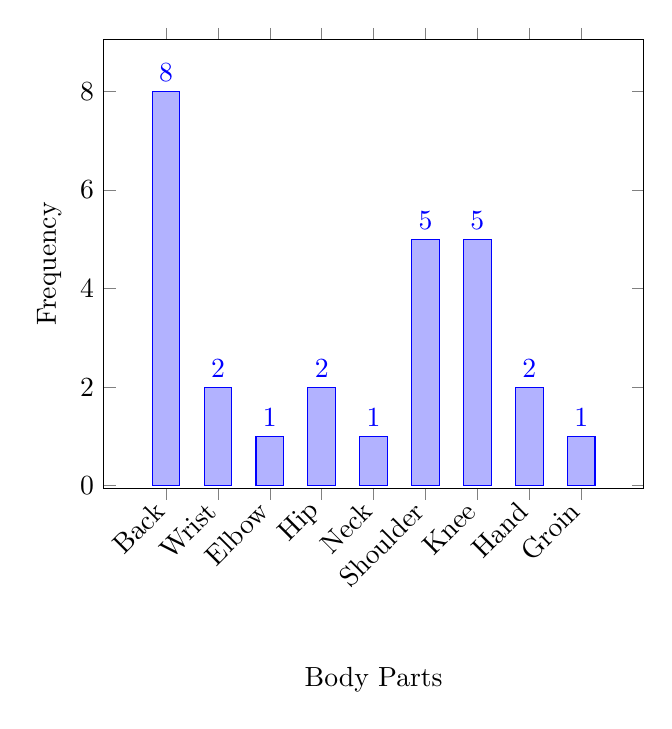
\begin{tikzpicture}
\begin{axis}[
    ybar,
    enlargelimits=0.15,
    ylabel={Frequency},
    xlabel={Body Parts},
    symbolic x coords={Back, Wrist, Elbow, Hip, Neck, Shoulder, Knee, Hand, Groin},
    xtick=data,
    nodes near coords,
    nodes near coords align={vertical},
    xlabel style={yshift=-20pt}, % Adjust the y position of the x-axis label
    x tick label style={rotate=45, anchor=east}, % Rotate x-axis labels
    ]
\addplot coordinates {(Back,8) (Wrist,2) (Elbow,1) (Hip,2) (Neck,1) (Shoulder,5) (Knee,5) (Hand,2) (Groin,1)};
\end{axis}
\end{tikzpicture}
        \end{center}

        \bigbreak \noindent 
        \textbf{Comparing Two Sets of Data}
        \bigbreak \noindent 
        First, determine the relative frequencies of each category for each year. To construct side-by-side bar graphs, draw two bars for each category of data.

        \bigbreak \noindent 
        \textbf{Horizontal Bars}
        \bigbreak \noindent 
        Bar graphs may also be drawn with horizontal bars. Horizontal bars are preferable when category names are lengthy. For example, Figure 4 uses horizontal bars to display the same data as in Figure 3.

        \bigbreak \noindent \bigbreak \noindent 
        \textbf{\textit{\underline{Construct Pie-Graphs}}}
        \bigbreak \noindent 
        Pie charts are typically used to present the relative frequency of qualitative data. In most cases, the data are nominal, but ordinal data can also be displayed in a pie chart.

        \bigbreak \noindent 
        \textbf{When should a Bar Graph or Pie Chart be Used?}
        \bigbreak \noindent 
        Pie chart are useful for showing the division of all possible values of a qualitative variable into its parts.
        \bigbreak \noindent 
        However, because angles are often hard to judge in pie charts, they are not as useful in comparing two specific values of the qualitative variable. 
        \bigbreak \noindent 
        Instead, the emphasis is on comparing the part to the whole.
        \bigbreak \noindent 
        Bar graphs are useful are useful when we want to compare the different parts, not necessarily the parts to the whole.

        \bigbreak \noindent 
        Since bars are easier to draw and compare, some forgo pie charts in favor of Pareto charts when comparing parts to the whole.

        \pagebreak \bigbreak \noindent
        \subsection{2.2: Organizing Quantitative Data: The Popular Displays}
        \bigbreak \noindent 
        \textbf{\textit{\underline{Learning Objectives For This Section:}}}
        \begin{enumerate}
            \item \textbf{Organize Discrete Data in Tables}
            \item \textbf{Construct Histograms of Discrete Data}
            \item \textbf{Organize Continuous Data in Tables}
            \item \textbf{Construct Histograms of Continuous Data}
            \item \textbf{Draw Dot Plots}
            \item \textbf{Identify the Shape of a Distribution}
        \end{enumerate}
        \bigbreak \noindent 
        \textbf{Vocab:}
        \begin{itemize}
            \item A \textbf{histogram} is constructed by drawing rectangles for each class of data. The height of each rectangle is the frequency or relative frequency of the class. The width of each rectangle is the same, and the rectangles touch each other.
            \item \textbf{Classes: } The Categories in which data is grouped
            \item \textbf{lower class limit:} the smallest value within the class 
            \item \textbf{upper class limit:} the largest value within the class 
            \item \textbf{Class Width: }  is the difference between consecutive lower class limits.
            \item A table is \textbf{open ended} if the first class has no lower class limit or the last class has no upper class limit
            \item We draw a \textbf{dot plot} by placing each observation horizontally in increasing order and placing a dot above the observation each time it is observed.
            \item \textbf{uniform distribution:} frequency of each value of the variable is evenly spread across the values of the variable. 
            \item \textbf{bell-shaped distribution:} highest frequency occurs in the middle and frequencies tail off to the left and right of the middle.
            \item \textbf{skewed right:} the tail to the right of the peak is longer than the tail to the left of the peak
            \item \textbf{skewed left:} tail to the left of the peak is longer than the tail to the right of the peak.
        \end{itemize}


        \bigbreak \noindent \bigbreak \noindent 
        \textbf{\textit{\underline{Organize Discrete Data in Tables}}}
        \bigbreak \noindent 
        Use the values of the discrete variable to create the classes when the number of distinct data values is small. The approach to summarizing the data is similar to that of constructing frequency or relative frequency distributions from qualitative data where the categories of data are determined by the actual observations.

        \bigbreak \noindent \bigbreak \noindent 
        \textbf{\textit{\underline{Construct Histograms of Discrete Data}}}
        \bigbreak \noindent 
        The \textit{histogram}, a graph used to present quantitative data, is similar to the bar graph.
        \bigbreak \noindent 
        The value of each category of data (number of customers) is on the horizontal axis and the frequency or relative frequency is on the vertical axis. Draw rectangles of equal width centered at the value of each category. 


        \bigbreak \noindent \bigbreak \noindent \bigbreak \noindent \bigbreak \noindent \bigbreak \noindent \bigbreak \noindent \bigbreak \noindent \bigbreak \noindent \bigbreak \noindent \bigbreak \noindent \bigbreak \noindent 
        \begin{center}
            \textbf{Histogram (Left) vs Bar Graph (Right)}
        \end{center}
        \bigbreak \noindent \bigbreak \noindent 
        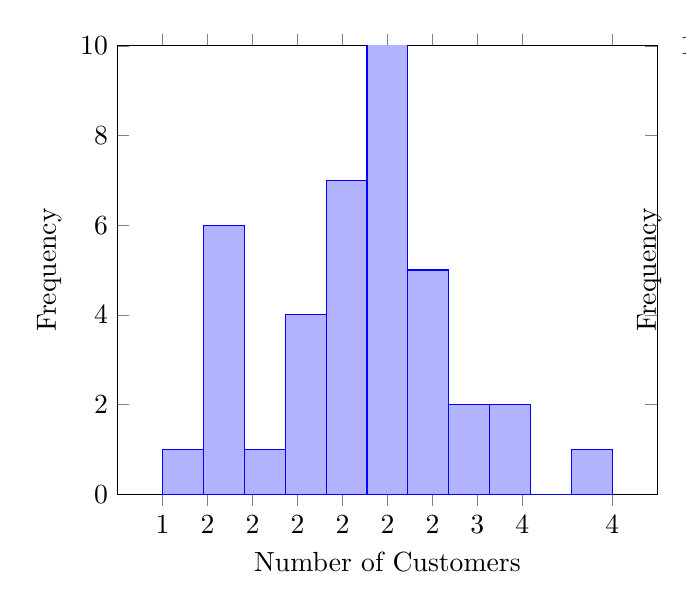
\begin{tikzpicture}
        \begin{axis}[
            ybar,
            ylabel={Frequency},
            xlabel={Number of Customers},
            ymin=0,
            ymax=10,
            xtick={1,2,3,4,5,6,7,8,9,11},
            xticklabels={1,2,2,2,2,2,2,3,4,4,4,4,5,5,5,5,5,5,5,6,6,6,6,6,6,6,6,6,6,7,7,7,7,7,8,8,9,9,11},
            enlarge x limits=0.1,
            ]
        \addplot+ [hist={bins=11}]
        table[row sep=\\,y index=0] {
        data\\
        1\\
        2\\
        2\\
        2\\
        2\\
        2\\
        2\\
        3\\
        4\\
        4\\
        4\\
        4\\
        5\\
        5\\
        5\\
        5\\
        5\\
        5\\
        5\\
        6\\
        6\\
        6\\
        6\\
        6\\
        6\\
        6\\
        6\\
        6\\
        6\\
        6\\
        7\\
        7\\
        7\\
        7\\
        7\\
        8\\
        8\\
        9\\
        9\\
        11\\
        };

        \end{axis}
        \hspace{3in}
        \begin{axis}[
            ybar,
            ylabel={Frequency},
            xlabel={Number of Customers},
            ymin=0,
            ymax=10,
            xtick=data,
            symbolic x coords={1,2,3,4,5,6,7,8,9,11},
            enlarge x limits=0.1,
            ]
        \addplot coordinates {
            (1,1)
            (2,6)
            (3,1)
            (4,4)
            (5,7)
            (6,10)
            (7,5)
            (8,2)
            (9,2)
            (11,1)
        };
        \end{axis}
        \end{tikzpicture}

        \bigbreak \noindent \bigbreak \noindent 
        \textbf{\textit{\underline{Organize Data Into Tables:}}}
        \bigbreak \noindent 
        When a data set consists of a large number of different discrete data values or when a data set consists of continuous data, create classes by using intervals of numbers.
        \bigbreak \noindent 
        \textbf{StatCrunch Steps:}
        \begin{itemize}
            \item Data $>$ Bin
            \item Select the column containing the data
            \item Choose a starting point and a binwidth (or automatic)
            \item Stat $>$ Tables $>$ Frequency (With newly generated data)
        \end{itemize}

        \bigbreak \noindent \bigbreak \noindent 
        \textbf{\textit{\underline{Draw Histograms of Continuous Data:}}}
        \bigbreak \noindent 
        \textbf{StatCrunch Steps:}
        \begin{itemize}
            \item Graph $>$ Histogram
            \item Select Data
            \item Input Bins
        \end{itemize}
        \textbf{Constructing Histograms Is Somewhat of an Art Form}
        \bigbreak \noindent 
        There is no one correct frequency distribution for a particular set of data. However, some frequency distributions better illustrate patterns within the data than others. So constructing frequency distributions is somewhat of an art form. Use the distribution that seems to provide the best overall summary of the data.
        \bigbreak \noindent 
         When the data set is small, we usually want fewer classes. When the data set is large, we usually want more classes. The larger the class width, the fewer the classes in a frequency distribution. Use the following guidelines to help determine an appropriate lower class limit of the first class and class width.

         \begin{mdframed}
             \textbf{\textit{\underline{Guidelines for Determining the Lower Class Limit of the First Class and Class Width}}}
             \bigbreak \noindent 
             \textbf{Choosing the Lower Class Limit of the First Class:}
             \bigbreak \noindent 
             Choose the smallest observation in the data set or a convenient number slightly smaller than the smallest observation in the data set.
             \bigbreak \noindent 
             \textbf{Determining the Class Width:}
             \begin{itemize}
                 \item Decide on the number of classes. Generally, there should be between 5 and 20  classes. The smaller the data set, the fewer the classes.
                 \item Determine the class width by computing
                     \begin{align*}
                         Class\ Width \approx \frac{Largest\ data\ value - smallest\ data\ value}{number\ of\ classes}
                     .\end{align*}
                \item Round the value to a convenient number. Rounding up may result in fewer classes than were originally intended, while rounding down may result in more class than originally intended.
             \end{itemize}
         \end{mdframed}

         \bigbreak \noindent \bigbreak \noindent 
         \textbf{\textit{\underline{Drawing Dot Plots:}}}
         \bigbreak \noindent 
         We draw a dot plot by placing each observation horizontally in increasing order and placing a dot above the observation each time it is observed.

         \bigbreak \noindent \bigbreak \noindent 
         \textbf{\textit{\underline{Identify the Shape of a Distribution:}}}
        \begin{figure}[ht]
            \centering
            \incfig{sr}
            \label{fig:sr}
        \end{figure}

        \pagebreak \bigbreak \noindent
        \subsection{2.4: Graphical Misrepresentations of Data}
        \bigbreak \noindent 
        \textbf{\textit{\underline{Learning Objectives For This Section:}}}
        \begin{enumerate}
            \item \textbf{Describe What Can Make a Graph Misleading or Deceptive}
        \end{enumerate}

        \bigbreak \noindent 
        \textbf{\textit{\underline{Describe What Can Make a Graph Misleading or Deceptive}}}
        \bigbreak \noindent 
        Statistics is the only science that enables different experts using the same figures to draw different conclusions.
        \bigbreak \noindent 
        Graphs that mislead unintentionally create an incorrect impression
        \bigbreak \noindent 
        Graphs that are deceptive purposely create an incorrect impression
        \bigbreak \noindent 
        \textbf{Most common graphical misrepresentations of data:}
        \begin{itemize}
            \item \textbf{Scale}
            \item \textbf{Inconsistent Scale}
            \item \textbf{Misplaced Origin}
        \end{itemize}
        \textbf{Guidelines for Constructing Good Graphics}
        \begin{itemize}
            \item Label and name the axes clearly, providing explanations if needed. Include units of measurement and a data source when appropriate.
            \item Include a meaningful title on the graph.
            \item Avoid distortion. Never lie about the data.
            \item Minimize the amount of white space in the graph. Use the available space to let the data stand out. If you truncate the scales, clearly indicate this to the reader.
            \item Avoid clutter, such as excessive gridlines and unnecessary backgrounds or pictures. Don't distract the reader from the data.
            \item Avoid three dimensions. Three-dimensional charts may look nice, but they distract the reader and often lead to misinterpretation of the graphic.
            \item Do not use more than one design in the same graphic. Sometimes graphs use a different design in one portion to draw attention to that area. Don't try to force the reader to a specific part of the graph. Let the data speak for themselves.
            \item Avoid relative graphs that do not contain data or scales.
            \item One final point to make. When reading graphs, look at the source of the data represented in the graphic. Often, a group with an agenda will conduct allegedly unbiased studies and report the results that support their position. Always "consider the source" and any possible hidden agendas they may have when reading graphics.
        \end{itemize}

        \pagebreak \bigbreak \noindent
        \section{Chapter 3:}
        \bigbreak \noindent 
        \subsection{3.1: Measures of Central Tendency}
        \bigbreak \noindent 
        \textbf{\textit{\underline{Learning Objectives For This Section:}}}
        \begin{enumerate}
            \item \textbf{Determine the Arithmetic Mean of a Variable from Raw Data}
            \item \textbf{Determine the Median of a Variable from Raw Data}
            \item \textbf{Explain What It Means for a Statistic to be Resistant}
            \item \textbf{Determine the Mode of a Variable from Raw Data}
        \end{enumerate}
        \bigbreak \noindent 
        \textbf{Vocab:}
        \begin{itemize}
            \item \textbf{The arithmetic mean} of a variable is computed by adding all the values of the variable in the data set and dividing by the number of observations.
            \item \textbf{The population arithmetic mean}, $\mu$, (pronounced "mew"), is a parameter that is computed using data from all the individuals in a population.
                \begin{align*}
                    \mu = \frac{x_{1}+x_{2} + x_{N}}{N} = \frac{\summation{}{}x_{i}}{N}
                .\end{align*}
            \item \textbf{The sample arithmetic mean}, $\bar{x}$ (pronounced x-bar"), is a statistic that is computed using data from individuals in a sample.
                \begin{align*}
                    \bar{x} = \frac{x_{1}+x_{2} + x_{n}}{n} = \frac{\summation{}{}x_{i}}{n}
                .\end{align*}
            \item \textbf{The median} of a variable is the value that lies in the middle of the data when arranged in ascending order. We use $M$  to represent the median.
            \item A numerical summary of data is said to be \textbf{resistant} if observations that are extreme (very large or small) relative to the data do not affect its value substantially.
                \begin{itemize}
                    \item So the median is resistant, but the mean is not resistant.
                \end{itemize}
            \item \textbf{The mode} of a variable is the observation of the variable that occurs most frequently in the data set.
                \begin{itemize}
                    \item If no observation occurs more than once, we say that the data have \textbf{no mode}.
                \end{itemize}
            \item \textbf{Bimodal:} If the data has two modes
            \item \textbf{Multimodal:} If the data has more than two modes
            \item A numerical summary of data is said to be \textbf{resistant} if observations that are extreme (very large or small) relative to the data do not affect its value substantially.
                \begin{itemize}
                    \item So the median is resistant, but the mean is not resistant.
                \end{itemize}
        \end{itemize}

        \bigbreak \noindent \bigbreak \noindent 
        \textbf{\textit{\underline{Determine the Arithmetic Mean of a Variable from Raw Data:}}}
        \bigbreak \noindent 
        Throughout this course, we agree to round the mean to one more decimal place than that in the raw data.
        \bigbreak \noindent 
        If $x_{1}, x_{2},...,x_{N}$ are the $N$  observations of a variable from a population, then the population mean, $\mu$  (pronounced "mew"), is:
        \begin{align*}
            \mu = \frac{x_{1} + x_{2} + ... + x_{N}}{N} = \frac{\summation{}{}x_{i}}{N}
        .\end{align*}
        \bigbreak \noindent 
        If $x_{1}, x_{2},...,x_{n}$ are the $n$  observations of a variable from a sample, then the sample mean, $\overline{x}$  (pronounced "x-bar"), is:
        \begin{align*}
            \overline{x} = \frac{x_{1} + x_{2} + ...+ x_{n}}{n} = \frac{\summation{}{}x_{i} }{n}
        .\end{align*}
        \bigbreak \noindent 
        \begin{mdframed}
          \textbf{Example: The table shows the first exam scores of the ten students enrolled in Introductory Statistics. }
          \begin{center}
          \begin{tabular}{|c|c|}
            \hline
            \textbf{Student} & \textbf{Score} \\
            \hline
            1. Michelle & 82 \\
                \hline
            2. Ryanne & 77 \\
                \hline
            3. Bilal & 90 \\
                \hline
            4. Pam & 71 \\
                \hline
            5. Jennifer & 62 \\
                \hline
            6. Dave & 68 \\
                \hline
            7. Joel & 74 \\
                \hline
            8. Sam & 84 \\
                \hline
            9. Justine & 94 \\
                \hline
            10. Juan & 88 \\
            \hline
            \end{tabular}
          \end{center}
          \bigbreak \noindent 
          \begin{enumerate}[label=\alph*.)]
          \item \textbf{Compute the population mean, $\mu $}
          \item \textbf{Find a simple random sample of size $n=4$ students}
          \item \textbf{compute the sample mean, $\overline{x} $}
          \end{enumerate}
          \bigbreak \noindent 
          \textbf{a.)} To compute the population mean, $\mu$,  add all the data values (test scores) and then divide by the number of individuals in the population.
          \begin{align*}
              \frac{\summation{}{}x_{i}}{N}
          .\end{align*}
          \bigbreak \noindent 
          Since we know $N = 10$:
          \begin{align*}
              \summation{}{}x_{i} = 82+77+90+71+62+68+74+84+94+88 \\
              = 790
          .\end{align*}
          \bigbreak \noindent 
          Now:
          \begin{align*}
              \frac{790}{10} 
              = 79
          .\end{align*}
          \bigbreak \noindent 
          \textbf{Note:} Although it was not necessary in this problem, we will agree to round the mean to one more decimal place than that in the raw data.
          \bigbreak \noindent 
          \textbf{b.)} To find a simple random sample of size $n=4$, we will use a ti-84 calculator.
          \begin{align*}
              rand(1,10,4) = \{5,10,2,6\} \\
              = Jennifer,\ Juan,\ Ryanne,\ Dave
          .\end{align*}
          \bigbreak \noindent 
          \textbf{c.)} 
          \begin{align*}
              \frac{x_{5} + x_{10} + x_{2} + x_{6}}{4} \\
              = \frac{62 + 88 + 77 +68}{4} \\
              = 73.8
          .\end{align*}
          \bigbreak \noindent 
          \textbf{Note:} Notice that we rounded the sample mean to the nearest tenth (which is one more decimal point than the original data).
        \end{mdframed}

        \bigbreak \noindent 
        \textbf{\textit{\underline{Determine the Median of a Variable from Raw Data}}}
        \bigbreak \noindent 
        A second measure of central tendency is the median. To compute the median of a set of data, the data must be quantitative.
        \bigbreak \noindent 
        \textbf{Steps in Finding the Median of a Data Set:}
        \begin{enumerate}
            \item Arrange the data in ascending order.
            \item Determine the number of observations, $n $
            \item Determine the observation in the middle of the data set.
            \begin{itemize}
                \item  If the number of observations is odd, then the median is the data value exactly in the middle of the data set. That is, the median is the observation that lies in the  $\frac{n+1}{2} $ position.
                \item  If the number of observations is even, then the median is the mean of the two middle observations in the data set. That is, the median is the mean of the observations that lie in the $\frac{n}{2}$ and the $\frac{n}{2} + 1 $ position.
            \end{itemize}
        \end{enumerate}
        \bigbreak \noindent 
        \begin{mdframed}
          \textbf{Example: Determining the Median of a Data Set (Odd Number of Observations)}
          \begin{center}
              \begin{tabular}{|l|c|}
                \hline
                \textbf{Song Name} & \textbf{Length} \\
                \hline
                ``Sister Golden Hair'' & 201 \\
                \hline
                ``Black Water'' & 257 \\
                \hline
                ``Free Bird'' & 284 \\
                \hline
                ``The Hustle'' & 208 \\
                \hline
                ``Southern Nights'' & 179 \\
                \hline
                ``Stayin' Alive'' & 222 \\
                \hline
                ``We Are Family'' & 217 \\
                \hline
                ``Heart of Glass'' & 206 \\
                \hline
                ``My Sharona'' & 240 \\
                \hline
                \end{tabular}
          \end{center}
          \bigbreak \noindent 
          \textbf{Step 1.} Arrange the data in ascending order:
          \begin{align*}
              179,201,206,208,217,222,240,257,284
          .\end{align*}
          \bigbreak \noindent 
          \textbf{Step 2.} Notice that there are $n=9$ observations 
          \bigbreak \noindent 
          \textbf{Step 3.} Because $n$ is odd, the median is the observation exactly in the middle of the data set with the data written in ascending order. This value lies in the $5^{th} $ position.
          \begin{align*}
              M= 217
          .\end{align*}
        \end{mdframed}
        \bigbreak \noindent 
        \begin{mdframed}
          \textbf{Example: Determining the Median of a Data Set (Even Number of Observations)}
          \begin{center}
              \begin{tabular}{|c|c|}
                \hline
                \textbf{Student} & \textbf{Score} \\
                \hline
                1. Michelle & 82 \\
                \hline
                2. Ryanne & 77 \\
                \hline
                3. Bilal & 90 \\
                \hline
                4. Pam & 71 \\
                \hline
                5. Jennifer & 62 \\
                \hline
                6. Dave & 68 \\
                \hline
                7. Joel & 74 \\
                \hline
                8. Sam & 84 \\
                \hline
                9. Justine & 94 \\
                \hline
                10. Juan & 88 \\
                \hline
                \end{tabular}
          \end{center}
          \bigbreak \noindent 
          \textbf{Step 1.} Arrange the data in ascending order:
          \begin{align*}
            62,68,71,74,77,82,84,88,90,94
          .\end{align*}
          \bigbreak \noindent 
          \textbf{Step 2.} Notice there are $n=10$ observations
          \bigbreak \noindent 
          \textbf{Step 3.} Because $n$ is even, the median is the mean of the two middle observations, the fifth $\bigg(\frac{n}{2} = \frac{10}{2} = 5\bigg) $ and sixth $\bigg(\frac{n}{2} + 1 = \frac{10}{2} + 1 = 6\bigg) $  observations with the data written in ascending order. So the median is the mean of $77$ and $82$
          \begin{align*}
              M = \frac{77 + 82}{2} \\
              =79.5
          .\end{align*}
         \end{mdframed}

         \bigbreak \noindent \bigbreak \noindent 
         \textbf{\textit{\underline{Explain What It Means for a Statistic to be Resistant:}}}
         \bigbreak \noindent 
         Which measure of central tendency is better to use—the mean or the median? It depends.
         \bigbreak \noindent 
         \nt{The value of the mean can be impacted by a single observation.} 
         \bigbreak \noindent 
         You may be asking yourself, "Why would I ever compute the mean?" After all, the mean and median are close in value for symmetric data, and the median is the better measure of central tendency for skewed data. The reason we compute the mean is that much of statistical inference is based on the mean.
         \bigbreak \noindent \bigbreak \noindent \bigbreak \noindent \bigbreak \noindent \bigbreak \noindent \bigbreak \noindent \bigbreak \noindent \bigbreak \noindent \bigbreak \noindent \bigbreak \noindent \bigbreak \noindent \bigbreak \noindent \bigbreak \noindent \bigbreak \noindent \bigbreak \noindent \bigbreak \noindent \bigbreak \noindent \bigbreak \noindent 
         \begin{center}
             \textbf{Relation among the Mean, Median, and Distribution Shape}
         \end{center}
         \begin{center}
             \begin{tabular}{|l|l|}
                \hline
                \textbf{Distribution Shape} & \textbf{Mean versus Median} \\
                \hline
                Skewed left & Mean substantially smaller than median \\
                \hline
                Symmetric & Mean roughly equal to median \\
                \hline
                Skewed right & Mean substantially larger than median \\
                \hline
                \end{tabular}
         \end{center}
         \bigbreak \noindent 
         \nt{ A word of caution is in order. The relation between the mean, median, and skewness are guidelines. These guidelines tend to hold up well for continuous data, but when the data are discrete the rules can be easily violated. \\
             When the data set is skewed the median is the preferred measure of central tendency. \\
             When the data set is symmetric the mode is the preferred measure of central tendency. 
         }

         \bigbreak \noindent \bigbreak \noindent 
         \textbf{\textit{\underline{Determine the Mode of a Variable from Raw Data}}}
         \bigbreak \noindent 
         A third measure of central tendency is the \textbf{mode}, which can be computed for either quantitative or qualitative data.
         \begin{itemize}
             \item To compute the mode, tally the number of observations that occur for each data value.
             \item The data value that occurs most often is the mode.
             \item If no observation occurs more than once, we say that the data have no mode.
             \item A set of data can have no mode, one mode, or more than one mode.
         \end{itemize}

         \bigbreak \noindent \bigbreak \noindent 
         \textbf{\textit{\underline{Summary:}}}
         \bigbreak \noindent 
        \begin{figure}[ht]
            \centering
            \incfig{figure2}
            \label{fig:figure2}
        \end{figure}

        \pagebreak \bigbreak \noindent
        \subsection{3.2: Measures of Dispersion}
        \bigbreak \noindent 
        \textbf{\textit{\underline{Learning Objectives For This Section:}}}
        \begin{enumerate}
            \item \textbf{Determine the Range of a Variable from Raw Data}
            \item \textbf{Determine the Standard Deviation of a Variable from Raw Data}
            \item \textbf{Determine the Variance of a Variable from Raw Data}
            \item \textbf{Use the Empirical Rule to Describe Data That Are Bell-Shaped}
        \end{enumerate}
        \bigbreak \noindent 
        \textbf{Vocab:}
        \begin{itemize}
            \item \textbf{Dispersion:} Degree to which the data are spread out. 
            \item \textbf{Range:} The range, $r $, of a variable is the difference between the largest and smallest data value. That is,
                \begin{align*}
                    range = R = Largest\ data\ value- smallest\ data\ value
                .\end{align*}
                \textbf{Note:} Range is \textbf{not} resistant
            \item \textbf{Deviation:} a deviation refers to the difference between an individual data point and a central value, such as the mean or median. It represents how much a particular data point varies or deviates from the average or typical value in a data set. When can comopute a deviation with:
                \begin{align*}
                    Individual\ data\ point - mean
                .\end{align*}
                We call this calculation, "deviation about the mean"
                \bigbreak \noindent 
                \textbf{Note:} The sum of the deviations about the mean always equals zero
            \item \textbf{The population standard deviation} of a variable is the square root of the sum of squared deviations about the population mean divided by the number of observations in the population, $N$. The population standard deviation is symbolically represented by $\sigma$ (lowercase Greek sigma). The formula is given by:
                \begin{align*}
                    \sigma = \sqrt{\frac{(x_{1} - \mu)^{2} + (x_{2}-\mu)^{2}+...+(x_{N}-\mu)^{2}}{N}} \\
                    = \sqrt{\frac{\summation{}{}(x_{i}-\mu)^{2} }{N}}
                .\end{align*}
                \textbf{Note:} Standard Deviation is \textbf{not} resistant
            \item \textbf{The sample standard deviation}, $s $, of a variable is the square root of the sum of squared deviations about the sample mean divided by $n-1 $, where $n$  is the sample size. The formula is given as
                \begin{align*}
                    s = \sqrt{\frac{(x_{1} - \overline{x})^{2}+(x_{2}-\overline{x})^{2}+...+(x_{n}-\overline{x})^{2}}{n-1}}\\
                    = \sqrt{\frac{\summation{}{}(x_{i}-\overline{x})^{2}}{n-1}}
                .\end{align*}
                \textbf{Note:} Standard Deviation is \textbf{not} resistant
            \item  we call $n-1$ the \textbf{degrees of freedom} because the first $n-1 $  observations have freedom to be any value, but the $n^{th}$ observation has no freedom. It must be whatever value forces the sum of the deviations about the mean to equal zero.
            \item The variance of a variable is the square of the standard deviation.
                \begin{itemize}
                    \item  \textbf{The population variance} is \textbf{$\sigma^{2}$} 
                    \item \textbf{The Sample Variance} is $s^{2}$
                \end{itemize}
                \textbf{Note:} The units of measure in variance are squared values. So if the variable is measured in dollars, the variance is measured in dollars squared. This makes interpreting the variance difficult.
            \item \textbf{Coefficient of Variation:} The coefficient of​ variation, CV, is defined as the ratio of the standard deviation to the mean of a data set. The CV allows for a comparison in spread by describing the amount of spread per unit mean.
                \begin{align*}
                    cv = \frac{Standard\ Deviation}{Mean}
                .\end{align*}
            \textbf{Note:} When converting units of​ measure, the coefficient of variation is unchanged.
        \end{itemize}
        \bigbreak \noindent 
        measures of center (such as the mean) are not sufficient in describing distributions of data. We determine numerical measures of dispersion to quantify the spread of data. This section discusses three numerical measures of dispersion, or spread, of data: the range, standard deviation, and variance.
        \bigbreak \noindent \bigbreak \noindent 
        \textbf{\textit{\underline{Determine the Range of a Variable from Raw Data:}}}
        \begin{align*}
            range = R = Largest\ data\ value- smallest\ data\ value
        .\end{align*}
        \bigbreak \noindent 
        \textbf{Note:} Range is \textbf{not} resistant

        \bigbreak \noindent \bigbreak \noindent
        \textbf{\textit{\underline{Determine the Standard Deviation of a Variable from Raw Data:}}}
        \bigbreak \noindent 
        \begin{mdframed}
          \textbf{Example: Population Standard Deviation}
          \bigbreak \noindent 
          Consider the data:
          \bigbreak \noindent 
          \begin{center}
          \begin{tabular}{|l|c|}
              \hline
            \textbf{Student} & \textbf{Score} \\
            % \midrule
            1. Michelle & 82 \\
            \hline
            2. Ryanne & 77 \\
            \hline
            3. Bilal & 90 \\
            \hline
            4. Pam & 71 \\
            \hline
            5. Jennifer & 62 \\
            \hline
            6. Dave & 68 \\
            \hline
            7. Joel & 74 \\
            \hline
            8. Sam & 84 \\
            \hline
            9. Justine & 94 \\
            \hline
            10. Juan & 88 \\
            \hline
          \end{tabular}
        \end{center}
        \bigbreak \noindent 
        To use the formula:
        \begin{align*}
            \sigma = \sqrt{\frac{\summation{}{}(x_{i} - \mu)^{2}}{N}}
        .\end{align*}
        \bigbreak \noindent 
        We must first compute $\mu$:
        \begin{align*}
            \mu = \frac{\summation{}{}x_{i}}{N} \\
            = \frac{82 + 77 + 90 + 71 + 62 + 68 + 74 + 84 + 94 + 88}{10} \\
            = 79
        .\end{align*}
        \bigbreak \noindent 
        Now:
        \begin{align*}
            \sigma = \sqrt{\frac{(82-79)^{2}+(77-79)^{2}+...+(88-79)^{2}}{10}} \\
            = \sqrt{96.4\ Points^{2}} \\
            =9.8\ Points
        .\end{align*}
        \end{mdframed}

        \bigbreak \noindent 
        \pagebreak \bigbreak \noindent
        \begin{mdframed}
          \textbf{Example: Calculating Standard Deviation (Sample Standard Deviation)}
          \bigbreak \noindent 
          Consider the data:
          \begin{center}
              \begin{tabular}{|l|c|}
              \hline
            Name & Exam Scores	 \\
            \hline
            Jennifer & 62 \\  	
            \hline
            Juan & 88 \\
            \hline
            Ryanne & 77 \\
            \hline 
            Dave &  68 \\
            \hline
              \end{tabular}
          \end{center}
          \bigbreak \noindent 
          If:
          \begin{align*}
              s = \sqrt{\frac{\summation{}{}(x_{i} - \overline{x})^{2}}{n-1}}
          .\end{align*}
          \bigbreak \noindent 
          First, we must find $\overline{x}$:
          \begin{align*}
              \overline{x} = \frac{\summation{}{}x_{i}}{n} \\
              = \frac{62 + 88 + 77 + 68}{4} \\
              = 73.75
          .\end{align*}
          \bigbreak \noindent 
          Now that we have computed $\overline{x}$, we can use the standard deviation formula:
          \begin{align*}
              s = \sqrt{\frac{(62-73.25)^{2} + (88-73.25)^{2} + (77-73.25)^{2} + (68-73.25)^{2}}{4-1}} \\
              = \sqrt{128.25\ points^{2}} \\
              \approx  11.3
          .\end{align*}
          \bigbreak \noindent 
          Remember, round the sample standard deviation to one more decimal place than the raw data.
        \end{mdframed}

        \bigbreak \noindent \bigbreak \noindent 
        \textbf{Interpretations of the Standard Deviation}
        \bigbreak \noindent 
        How does the value of the standard deviation relate to the spread of the distribution?
        \bigbreak \noindent 
        Standard deviation represents the "typical" deviation from the mean. As such, the standard deviation may be used to judge whether a particular observation is "far away" from the mean of a data set. For example, is a measure of 31  cm far from 25 cm? It depends. If the standard deviation of the data is 6cm  cm, then the answer is no because 31  cm would be only 1  standard deviation from 25  cm. However, if the standard deviation of the data is 2  cm, then the answer is yes because 31 cm would be 3  standard deviations from 25  cm. \textbf{A good rule of thumb is to consider an observation "far away" if it is more than 2  standard deviations from the other observation (such as the mean).}
        \bigbreak \noindent
        So, when judging the unusualness of an observation, it is vital that you consider the underlying variation in the data as measured by the standard deviation.
        \bigbreak \noindent 
        When comparing two populations, the larger the standard deviation, the greater the dispersion, or spread, of the distribution provided the variable of interest from the two populations has the same unit of measure. The units of measure must be the same so that we are comparing "apples with apples." For example, \$100 is not the same as 100 japanese yen (because recently  was equivalent to about 114 yen)  yen). So a standard deviation of \$100  yen). So a standard deviation of 100 yen
        \bigbreak \noindent 
        The standard deviation is used to describe the spread in symmetric distributions (while the mean is used to describe the center of the distribution).

        \bigbreak \noindent 
        \nt{Higher Standard Deviation $=$ more dispersion.}

        \bigbreak \noindent \bigbreak \noindent 
        \textbf{\textit{\underline{Determine the Variance of a Variable from Raw Data}}}
        \bigbreak \noindent 
        The units of measure in variance are squared values. So if the variable is measured in dollars, the variance is measured in dollars squared. This makes interpreting the variance difficult.
        \bigbreak \noindent 
        We can compute the variance in one of two ways.
        \begin{enumerate}
            \item Compute the std. dev and then square the result
            \item The expression under the radical in the formula for standard deviation is the formula for variance. Therefore if we drop the radical in the standard deviation formula, we can compute the variance.
        \end{enumerate}
        \bigbreak \noindent 
        \nt{Using a rounded value of the standard deviation to obtain the variance results in a round-off error}

        \bigbreak \noindent 
        \textbf{Bias in the Variance and Standard Deviation}
        \bigbreak \noindent 
        The sample variance is obtained using the formula:
        \begin{align*}
            s^{2} = \frac{\summation{i=1}{n}(x_{i} - \overline{x})^{2}}{n-1}
        .\end{align*}
        What if we divided by $n$ instead of $n-1 $?  to obtain the sample variance, as one might expect? Then the sample variance would consistently underestimate the population variance. Whenever a statistic consistently underestimates a parameter, it is said to be biased. To obtain an unbiased estimate of the population variance, divide the sum of the squared deviations about the sample mean by $n-1 $
        \bigbreak \noindent 
        Unfortunately, the sample standard deviation given by the formula:
        \begin{align*}
            s = \sqrt{\frac{\summation{i=1}{n}(x_{i} - \overline{x})^{2}}{n-1}}
        .\end{align*}
         is not an unbiased estimate of the population standard deviation. In fact, it is not possible to provide an unbiased estimator of the population standard deviation for all distributions. The explanation is beyond the scope of this class (it has to do with the shape of the square root function). However, for the applications in this text, the bias is minor and does not impact results.

         \pagebreak \bigbreak \noindent
         \textbf{\textit{\underline{Use the Empirical Rule to Describe Data That Are Bell-Shaped}}}
         \bigbreak \noindent 
         If data have a distribution that is bell-shaped, the Empirical Rule can be used to determine the percentage of data that will lie within $k $ standard deviations of the mean.
         \bigbreak \noindent 
         \textbf{The Empirical Rule:}
         \bigbreak \noindent 
         If a distribution is roughly bell shaped, then
         \begin{itemize}
             \item approximately $68\% $ of the data within $1 $ standard deviation of the mean. That is, approximately $68\% $  of the data will lie between $\mu-1 \sigma $ and $\mu + 1 \sigma $ 
             \item approximately $95\% $ of the data within $2 $ standard deviation of the mean. That is, approximately $95\% $  of the data will lie between $\mu-2 \sigma $ and $\mu + 2 \sigma $ 
             \item approximately $99.7\% $ of the data within $3 $ standard deviation of the mean. That is, approximately $99.7\% $  of the data will lie between $\mu-3 \sigma $ and $\mu + 3 \sigma $ 
         \end{itemize}
         \bigbreak \noindent 
         \nt{The Empirical Rule can also be used based on sample data with $\overline{x} $ in place of $\mu$ and $s$ in place of $\sigma $}
         \pagebreak \bigbreak \noindent
         \subsection{3.3: Measures of Central Tendency and Dispersion from Grouped Data}
         \bigbreak \noindent 
         \textbf{\textit{\underline{Learning Objectives For This Section:}}}
         \begin{enumerate}
             \item \textbf{Approximate the Mean of a Variable from Grouped Data}
             \item \textbf{Compute the Weighted Mean}
             \item \textbf{Approximate the Standard Deviation from a Frequency Distribution}
         \end{enumerate}
         \bigbreak \noindent 
         \textbf{Vocab/Formulas:}
         \begin{itemize}
             \item \textbf{Class Midpoint:} The class midpoint is the sum of consecutive lower class limits divided by 2
             \item \textbf{Approximate Population Mean (if we do not have access to the original data, ie data has been grouped (classed) and frequency chart has already been made)}
                \begin{align*}
                    \mu =\frac{\sum x_i f_i}{\sum f_i} \\
                     =\frac{x_1 f_1+x_2 f_2+\cdots+x_n f_n}{f_1+f_2+\cdots+f_n}
                .\end{align*}
            where: $\quad x_i$ is the midpoint or value of the $i$ th class  \\
            $f_i$ is the frequency of the $i$ th class  \\
            $n$ is the number of classes
            \item \textbf{Approximate Sample Mean (if we do not have access to the original data, ie data has been grouped (classed) and frequency chart has already been made)}
                \begin{align*}
                    \overline{x} = \frac{\sum x_{i}f_{i}}{\sum f_{i}} \\
                     = \frac{x_{1}f_{1} + x_{2} f_{2} + ... +x_{n} f_{n}}{f_{1} + f_{2} + ... + f_{n}}
                .\end{align*}
            where: $\quad x_i$ is the midpoint or value of the $i$ th class  \\
            $f_i$ is the frequency of the $i$ th class  \\
            $n$ is the number of classes
            \item \textbf{The weighted mean}, $\overline{x}_{w}$, of a variable is found by multiplying each value of the variable by its corresponding weight, adding these products, and dividing this sum by the sum of the weights. It can be expressed using the formula
                \begin{align*}
                    \overline{x}_{w} = \frac{\sum w_{i}x_{i}}{w_{i}} = \frac{w_{1} + x_{1} + w_{2} + x_{2} + ... + w_{n} + x_{n}}{w_{1} + w_{2} + ... + w_{n}}
                .\end{align*}
                Where: \quad $w_{i}$ is the weight of the $i^{th}$ observation \\
                $x_{i}$ is the value of the $i^{th}$ observation.
            \item \textbf{Approximate Population Standard Deviation (if we do not have access to the original data, ie data has been grouped (classed) and frequency chart has already been made)}
                \begin{align*}
                    \sigma = \sqrt{\frac{\sum(x_{i} - \mu)^{2}f_{i}}{\sum f_{i}}}
                .\end{align*}
                Where: \quad  $x_{i}$ is the midpoint or value of the ith class \\
                $f_{i}$ is the frequency of the $i^{th}$ class
            \item \textbf{Approximate Sample Standard Deviation (if we do not have access to the original data, ie data has been grouped (classed) and frequency chart has already been made)}
                \begin{align*}
                    s = \sqrt{\frac{\sum(x_{i}-\overline{x})^{2}f_{i}}{\sum f_{i} -1}}
                .\end{align*}
                Where: \quad  $x_{i}$ is the midpoint or value of the ith class \\
                $f_{i}$ is the frequency of the $i^{th}$ class
         \end{itemize}

         \pagebreak \bigbreak \noindent
         \textbf{\textit{\underline{Approximate the Mean of a Variable from Grouped Data}}}
         \bigbreak \noindent 
         Because raw data cannot be retrieved from a frequency table, we assume that within each class, the mean of the data values is equal to the class midpoint. Then multiply the class midpoint by the frequency. This product is expected to be close to the sum of the data that lie within the class. Repeat the process for each class and add the results. This sum approximates the sum of all the data.
         \bigbreak \noindent 
         In each formula, $x_{1}$ $f_{1} $  approximates the sum of all the data values in the first class, $x_{2}f_{2} $  approximates the sum of all the data values in the second class, and so on. Notice that the formulas for the population mean and sample mean are essentially identical, just as they were for computing the mean from raw data.

         \bigbreak \noindent 
         \begin{mdframed}
           \textbf{Example: Approximating the Mean for Continuous Quantitative Data from a Frequency Distribution}
           \bigbreak \noindent 
           Consider the data:
           \begin{center}
               \begin{tabular}{|c|c|}
                    \hline
                    Class & Frequency \\
                    \hline
                    8--8.99 & 2 \\
                    \hline
                    9--9.99 & 2 \\
                    \hline
                    10--10.99 & 4 \\
                    \hline
                    11--11.99 & 1 \\
                    \hline
                    12--12.99 & 6 \\
                    \hline
                    13--13.99 & 13 \\
                    \hline
                    14--14.99 & 7 \\
                    \hline
                    15--15.99 & 3 \\
                    \hline
                    16--16.99 & 1 \\
                    \hline
                    17--17.99 & 0 \\
                    \hline
                    18--18.99 & 0 \\
                    \hline
                    19--19.99 & 1 \\
                    \hline
                    \end{tabular}
           \end{center}
           \bigbreak \noindent 
           First let's find $x_{i}$ (Midpoints)
           \begin{center}
               \begin{tabular}{|c|c|c|c|}
                    \hline
                    Interval & Frequency & Midpoint (Full Expression) & Midpoint (Simplified) \\
                    \hline
                    8--8.99 & 2 & $\frac{8 + 9}{2}$ & 8.5 \\
                    \hline
                    9--9.99 & 2 & $\frac{9 + 10}{2}$ & 9.5 \\
                    \hline
                    10--10.99 & 4 & $\frac{10 + 11}{2}$ & 10.5 \\
                    \hline
                    11--11.99 & 1 & $\frac{11 + 12}{2}$ & 11.5 \\
                    \hline
                    12--12.99 & 6 & $\frac{12 + 13}{2}$ & 12.5 \\
                    \hline
                    13--13.99 & 13 & $\frac{13 + 14}{2}$ & 13.5 \\
                    \hline
                    14--14.99 & 7 & $\frac{14 + 15}{2}$ & 14.5 \\
                    \hline
                    15--15.99 & 3 & $\frac{15 + 16}{2}$ & 15.5 \\
                    \hline
                    16--16.99 & 1 & $\frac{16 + 17}{2}$ & 16.5 \\
                    \hline
                    17--17.99 & 0 & $\frac{17 + 18}{2}$ & 17.5 \\
                    \hline
                    18--18.99 & 0 & $\frac{18 + 19}{2}$ & 18.5 \\
                    \hline
                    19--19.99 & 1 & $\frac{19 + 20}{2}$ & 19.5 \\
                    \hline
                    \end{tabular}
           \end{center}
           \bigbreak \noindent 
           Now we can proceed with the formula:
           \begin{align*}
               \overline{x} = \frac{\sum x_{i}f_{i}}{\sum f_{i}} 
           .\end{align*}
           \bigbreak \noindent 
           So:
           \begin{align*}
                   \sum x_{i}f_{i} &= (8.5 \times 2) + (9.5 \times 2) + (10.5 \times 4) + (11.5 \times 1) + (12.5 \times 6) \\
                &\quad+ (13.5 \times 13) + (14.5 \times 7) + (15.5 \times 3) + (16.5 \times 1) + (17.5 \times 0) \\
                &\quad+ (18.5 \times 0) + (19.5 \times 1) = 524 \\
                f_{i} &= 2 + 2 + 4 + 1 + 6 + 13 + 7 + 3 + 1 + 0 + 0 + 1 = 40 \\
            \end{align*}
            \bigbreak \noindent 
            Therefore:
            \begin{align*}
                \overline{x} = \frac{524}{40} \\
                =13.1
            .\end{align*}
            \bigbreak \noindent 
            Thus we can conclude that approximate mean is $13.1\%$
         \end{mdframed}

         \bigbreak \noindent 
         \textbf{Steps for StatCrunch:}
         \begin{itemize}
             \item Stat $>$ Summary Stats $>$ Grouped/Binned data
            \item \textbf{Midpoints Defined By The Average Of:} \rightarrow Consecutive Lower Limits

         \end{itemize}

         \bigbreak \noindent \bigbreak \noindent 
         \textbf{\textit{\underline{Compute the Weighted Mean}}}
         \bigbreak \noindent 
         When data values have different importance, or weights, associated with them, we compute the weighted mean. For example, grade point average is a weighted mean, with weights equal to the number of credit hours in each course. The value of the variable is equal to the grade converted to a point value. 
         \bigbreak \noindent 
         \begin{mdframed}
           \textbf{Example: Computing the Weighted Mean}
           \bigbreak \noindent 
           Consider the data:
           \begin{center}
               \begin{center}
                   \begin{tabular}{|l|c|c|}
                   \hline
                   Class & Credit Hours & Grade \\
                   	\hline
                   Statistics & 4 	  & A (4 Points) \\
                   	\hline
                   Sociology & 3 & B (3 Points) \\
                   	\hline
                   Psychology & 3 & A (4 Points) \\
                   	\hline
                   Computer Programming & 5 & C (2 Points) \\
                   \hline
                   Drama & 1 & A (4 Points) \\
                   \hline
                   \end{tabular}
               \end{center}
           \end{center}
           \bigbreak \noindent 
           So:
           \begin{align*}
               \overline{x}_{w} = \frac{\sum w_{i}x_{i}}{\sum w_{i}} = \frac{(4\cdot 4) + ( 3\cdot 3) +  (3 \cdot 4) + (5 \cdot 2) + (1 + 4) }{4 + 3 + 3 + 5 + 1} \\
               = \frac{51}{16} =3.19
           .\end{align*}
           \bigbreak \noindent 
           Therefore:
           \begin{align*}
               \frac{51}{16} \\
               = 3.19
           .\end{align*}
           \bigbreak \noindent 
           Thus, Marissa's grade-point average for her first semester is $3.19 $
           
         \end{mdframed}
         \pagebreak \bigbreak \noindent
         \textbf{Steps for finding weighted mean in statcrunch:}
         \bigbreak \noindent 
         \begin{enumerate}
             \item Stat $> $ Summary Stats $> $ Grouped/Binned Data  
         \end{enumerate}

         \bigbreak \noindent \bigbreak \noindent 
         \textbf{\textit{\underline{Approximate the Standard Deviation from a Frequency Distribution}}}
         \bigbreak \noindent 
         The procedure for approximating the standard deviation from grouped data is similar to that of finding the mean from grouped data. Because we do not have access to the original data, the standard deviation is approximate.
         \bigbreak \noindent 
         \begin{mdframed}
           \textbf{Example: Approximating the Standard Deviation from a Frequency Distribution}
           \bigbreak \noindent 
           Consider the data:
                                 \begin{center}
               \begin{tabular}{|c|c|c|c|}
                    \hline
                    Interval & Frequency & Midpoint (Full Expression) & Midpoint (Simplified) \\
                    \hline
                    8--8.99 & 2 & $\frac{8 + 9}{2}$ & 8.5 \\
                    \hline
                    9--9.99 & 2 & $\frac{9 + 10}{2}$ & 9.5 \\
                    \hline
                    10--10.99 & 4 & $\frac{10 + 11}{2}$ & 10.5 \\
                    \hline
                    11--11.99 & 1 & $\frac{11 + 12}{2}$ & 11.5 \\
                    \hline
                    12--12.99 & 6 & $\frac{12 + 13}{2}$ & 12.5 \\
                    \hline
                    13--13.99 & 13 & $\frac{13 + 14}{2}$ & 13.5 \\
                    \hline
                    14--14.99 & 7 & $\frac{14 + 15}{2}$ & 14.5 \\
                    \hline
                    15--15.99 & 3 & $\frac{15 + 16}{2}$ & 15.5 \\
                    \hline
                    16--16.99 & 1 & $\frac{16 + 17}{2}$ & 16.5 \\
                    \hline
                    17--17.99 & 0 & $\frac{17 + 18}{2}$ & 17.5 \\
                    \hline
                    18--18.99 & 0 & $\frac{18 + 19}{2}$ & 18.5 \\
                    \hline
                    19--19.99 & 1 & $\frac{19 + 20}{2}$ & 19.5 \\
                    \hline
                    \end{tabular}
           \end{center}
           \bigbreak \noindent 
           Next, we can find $\overline{x} $:
           \begin{align*}
               &\sum x_{i}f_{i} =  (8.5\cdot 2) + (9.5\cdot 2) + (10.5 \cdot 4) + (11.5 \cdot 1) + (12.5 \cdot 6) \\
               &+ (13.5\cdot 13) + (14.5\cdot 7) + (15.5\cdot 3) + (16.5\cdot 1) + (19.5\cdot 1) \\
               &=524 \\
           .\end{align*}
           \begin{align*}
               \sum f_{i} = 2+2+4+1+6+13+7+3+1+1 \\
               = 40 \\
               \overline{x} = \frac{\sum x_{i}f_{i}}{\sum f_{i}} = \frac{524}{40} \\ = 13.1
           .\end{align*}
           \bigbreak \noindent 
           Now:
           \begin{align*}
               \sum (x_{i} - \overline{x}_{i})^{2}f_{i} &= ((8.5 - 13.1)^{2}\cdot 2) + ((9.5 - 10.33)^{2} \cdot 2) + ((10.5-10.33)^{2}\cdot 4) \\
                                               & +((11.5-13.1)^{2}\cdot 1) + ((12.5-10.33)^{2}\cdot 6) + ((13.5-10.33)^{2}\cdot 13) \\
                                               &+((14.5-13.1)^{2}\cdot 7) + ((15.5-10.33)^{2}\cdot 3) + ((16.5-10.33)^{2}\cdot 1) \\
                                               &+ ((19.5-13.1)^{2}\cdot 1) \\
                                               &= 185.6
           .\end{align*}
           And:
           \begin{align*}
               \sum f_{i} = 2+2+4+1+6+13+7+3+1+1 \\
               =40 
           .\end{align*}
           \bigbreak \noindent 
           Finally:
           \begin{align*}
               \sigma = \sqrt{\frac{185.6}{40-1}} \\
               =2.182
           .\end{align*}
           \bigbreak \noindent 
           Thus, The approximate standard deviation of the five-year rate of return is $2.182\% $
         \end{mdframed}

         \pagebreak \bigbreak \noindent
         \subsection{3.4: Measures of Position }
         \bigbreak \noindent 
         \textbf{\textit{\underline{Learning Objectives For This Section:}}}
         \begin{enumerate}
             \item \textbf{Determine and Interpret z-Scores}
             \item \textbf{Interpret Percentiles}
             \item \textbf{Determine and Interpret Quartiles}
             \item \textbf{Determine and Interpret the Interquartile Range}
             \item \textbf{Check a Set of Data for Outliers}
         \end{enumerate}
         \bigbreak \noindent 
         \textbf{Vocab:}
         \begin{itemize}
             \item \textbf{The z-score} represents the distance that a data value is from the mean in terms of the number of standard deviations. We find it by subtracting the mean from the data value and dividing this result by the standard deviation.
                 \begin{itemize}
                     \item \textbf{Population Z-score}
                 \end{itemize}
                 \begin{align*}
                      z = \frac{x - \mu}{\sigma}
                 .\end{align*}
                 \begin{itemize}
                     \item \textbf{Sample Z-score}
                 \end{itemize}
                 \begin{align*}
                     z =\frac{x-\overline{x}}{s}
                 .\end{align*}
                 \textbf{Note:} The Z-score is unitless. It has mean  0 and a standard deviation of 1 \\
                 \textbf{Round z-scores to the nearest hundredth}
             \item  The median is a special case of a general concept called the \textbf{percentile.}
             \item \textbf{the $k^{th}$  percentile,} denoted $P_{k} $,  of a set of data is a value such that $k $  percent of the observations are less than or equal to the value.
                \item The most common percentiles are \textbf{quartiles}, which divide data sets into fourths, or four equal parts.
                \item The \textbf{interquartile range, IQR,} is the range of the middle $50\% $  of the observations in a data set. That is, the IQR is the difference between the first and third quartiles and is found using this formula  
                    \begin{align*}
                        IQR = Q_{3} - Q_{1}
                    .\end{align*}
                \item \textbf{Outliers:} When analyzing data, we must check for extreme observations, called outliers. Outliers can occur by chance, because of errors in the measurement of a variable, during data entry, or from errors in sampling.
                \item \textbf{Fences} serve as cutoff points for determining outliers.
                    \begin{align*}
                        Lower\ Fence\ = Q_{1} - 1.5\cdot IQR \\
                        Upper\ Fence\ = Q_{3} + 1.5\cdot IQR
                    .\end{align*}


         \end{itemize}

         \pagebreak \bigbreak \noindent
         \textbf{\textit{\underline{Determine and Interpret z-scores:}}}
         \bigbreak \noindent 
       If a data value is larger than the mean, the z-score is positive. If a data value is smaller than the mean, the z-score is negative. If the data value equals the mean, the -score is zero. A z-score measures the number of standard deviations an observation is above or below the mean. For example, a  z-score of 1.24 means the data value is 1.24  standard deviations above the mean. A z-score of -2.31  means the data value is 2.31 standard deviations below the mean.
       \bigbreak \noindent 
          \begin{mdframed}
           \textbf{Example: Z-score}
           \bigbreak \noindent 
              In a certain city, the average​ 20- to 29-year old man is 69.8  inches​ tall, with a standard deviation of 3.1  ​inches, while the average​ 20- to​ 29-year old woman is 64.5  inches​ tall, with a standard deviation of 3.8  inches. Who is relatively​ taller, a​ 75-inch man or a​ 70-inch woman?
              \bigbreak \noindent 
                First, let's calculate the z-score of the man. We know that $\overline{x} = 69.8$ and $s = 3.1$, so:
                \begin{align*}
                    z = \frac{75-69.8}{3.1} \\
                    =1.68
                .\end{align*}
                \bigbreak \noindent 
                Now let's calculate the z-score of the women.
                \begin{align*}
                    z = \frac{70-64.5}{3.8} \\
                    =1.45
                .\end{align*}
                \bigbreak \noindent 
                Thus, we can conclude:
                The​ z-score for the 1.68​, is larger than the​ z-score for the woman, 1.45, so he  is relatively taller.
         \end{mdframed}

         \bigbreak \noindent \bigbreak \noindent 
         \textbf{\textit{\underline{Interpret Percentiles}}}
         \bigbreak \noindent 
         Percentiles divide a set of data, written in ascending order, into 100 parts such that 99  percentiles can be determined. For example, $P_{1}$  divides the bottom 1\%  divides the bottom 99\%, $P_{2} $  divides the bottom 2\%  of the observations from the top 98\%, and so on.
         \bigbreak \noindent 
         Percentiles are used to give the relative standing of an observation. Many standardized exams, such as the SAT, use percentiles to let students know how they scored on the exam in relation to all others who took the exam.

         \bigbreak \noindent \bigbreak \noindent 
         \textbf{\textit{\underline{Interpret Quartiles:}}}
         \bigbreak \noindent 
         \textbf{Steps for finding Quartiles}
         \begin{enumerate}
             \item Arrange the data in ascending order.
             \item Determine the median, $M $, Determine the median, $Q_{2}$
             \item Divide the data set into two halves: the observations less than $M$  and the observations greater than $M$  The first quartile, $Q_{1}$  is the median of the bottom half, and the third quartile, $Q_{3}$  is the median of the top half. Do not include $M$ in these halves.
         \end{enumerate}

         \pagebreak \bigbreak \noindent
         \bigbreak \noindent 
         \begin{mdframed}
           \textbf{Example: Find the quartiles}
           \bigbreak \noindent 
           Consider the data:
           \begin{center}
               2,4,6,8,10,12,14,16,18
           \end{center}
           \bigbreak \noindent 
           So we find $Q_{2}$ by finding the median of the entire data set:
           \begin{align*}
               Q_{2} = M = \frac{n+1}{2} = \frac{10}{2} = 5  \\
               = 10
           .\end{align*}
           \bigbreak \noindent 
           Now we can find $Q_{1}$ and $Q_{3}$ by dividing the data set into two sets at $Q_{2}$:
           \begin{align*}
               L_{1} = 2,4,6,8,10 \quad L_{2} = 10,12,14,16,18
           .\end{align*}
           \bigbreak \noindent 
           Now:
           \begin{align*}
               Q_{1} = M_{L_{1}} = \frac{n+1}{2} = \frac{6}{2} = 3 \\
               =6
           .\end{align*}
           \begin{align*}
               Q_{3} = M_{L_{2}} = \frac{n+1}{2} = \frac{6}{2} =3 \\
               =14
           .\end{align*}
           \bigbreak \noindent 
           Thus:
           \begin{align*}
               Q_{1} = 6 \\
               Q_{2} = 10 \\
               Q_{3} = 14
           .\end{align*}
           \bigbreak \noindent 
           Which means we can conclude:
           \begin{align*}
               25\% \leq 6 \quad 75\% \geq 6 \\
               50\% \leq 10 \quad 50\% \geq 10 \\
               75\% \leq 14 \quad 25\% \geq 14
           .\end{align*}
       \end{mdframed}

       \pagebreak \bigbreak \noindent
       \bigbreak \noindent 
       \begin{mdframed}
         \textbf{Example: Find the quartiles:}
         \bigbreak \noindent 
         consider the data:
         \begin{center}
             $d_{18}$  =  \$ 180, \$189, \$370, \$618, \$735, \$802, \$1185, \$1414, \$1657,\\ 
             \$1953, \$2332, \$2336, \$3461, \$4668, \$6751, \$9908, \$10,034, \$21,147
         \end{center}
         \bigbreak \noindent 
         First we find $Q_{2} = M $:
         \begin{align*}
             Q_{2} = M = \frac{d_{\frac{n}{2}} + d_{\frac{n}{2}+1}}{2} = \frac{1657 + 1953}{2} = \$1805
         .\end{align*}
         \bigbreak \noindent 
         Now we split the data into two halves:
         \begin{align*}
             &L_{1} = \$180, \$189, \$370, \$618, \$735, \$802, \$1185, \$1414, \$1657 \\ &L_{2} = \$1953, \$2332, \$2336, \$3461, \$4668, \$6751, \$9908, \$10,034, \$21,147
         .\end{align*}
         \bigbreak \noindent 
         Thus:
         \begin{align*}
             Q_{1} = M_{L_{1}} = \frac{n+1}{2} = \frac{10}{2} = 5 \\
             = \$735
         .\end{align*}
         \begin{align*}
             Q_{2} = M_{L_{2}} = \frac{n+1}{2} = \frac{10}{2} = 5 \\
             = \$4668
         .\end{align*}
       \end{mdframed}

       \bigbreak \noindent 
       \textbf{Steps for finding quartiles in StatCrunch:}
       \begin{enumerate}
           \item Stat $> $ Summary Stats $> $ Columns 
            \item Select Column
            \item Select Median, $Q_{1}$, and $Q_{3} $
       \end{enumerate}


       \bigbreak \noindent \bigbreak \noindent 
       \textbf{\textit{\underline{Determine and Interpret the Interquartile Range}}}
       \bigbreak \noindent 
       So far we have discussed three measures of dispersion: range, standard deviation, and variance. None of these measures of dispersion are resistant . Quartiles, however, are resistant. For this reason, quartiles are used to define a resistant measure of dispersion.
       \bigbreak \noindent 
       The interpretation of the interquartile range is the range of the middle $50\% $ of the data. The more spread a set of data has, the higher the interquartile range will be. The interquartile range, IQR, is a resistant measure of dispersion.

       \pagebreak \bigbreak \noindent
       \textbf{Deciding Which Measure of Central Tendency and Dispersion to Report:}
       \bigbreak \noindent 
       \begin{center}
           \begin{tabular}{|l|l|l|}
            \hline
            Shape of Distribution & Measure of Central Tendency & Measure of Dispersion \\
            \hline
            Symmetric & Mean & Standard Deviation \\
            \hline
            Skewed Left or Skewed Right & Median & Interquartile Range \\
            \hline
            \end{tabular}
       \end{center}
       \bigbreak \noindent 
       \nt{For the remainder of this course, the phrase "describe the distribution" will mean to describe its shape (skewed left, skewed right, or symmetric), its center (mean or median), and its spread (standard deviation or interquartile range).}

       \bigbreak \noindent 
       \textbf{Resistant Measures of Central Tendency:}
       \begin{itemize}
           \item \textbf{Median}
       \end{itemize}
      \textbf{Non-Resistant Measures of Central Tendency:}
      \begin{itemize}
          \item \textbf{Mean}
          \item \textbf{Mode}
      \end{itemize}
      \bigbreak \noindent 
      \textbf{Resistant Measures of Dispersion:}
      \begin{itemize}
          \item \textbf{Quartiles}
      \end{itemize}
      \bigbreak \noindent 
    \textbf{Non-Resistant Measures of Dispersion:}
    \begin{itemize}
        \item \textbf{Range.}
        \item \textbf{Standard Deviation.}
        \item \textbf{Variance.}
    \end{itemize}

    \bigbreak \noindent \bigbreak \noindent 
    \textbf{\textit{\underline{Check a Set of Data for Outliers}}}
    \bigbreak \noindent 
    When analyzing data, we must check for extreme observations, called outliers. Outliers can occur by chance, because of errors in the measurement of a variable, during data entry, or from errors in sampling.
    \bigbreak \noindent 
    Outliers aren't always due to error or chance. Sometimes extreme observations are common within a population. For example, suppose we wanted to estimate the mean price of a European car. We might take a random sample of size 5 from the population of all European cars. If our sample included a Ferrari F430 Spider (approximately \$175,000)), it probably would be an outlier because this car costs much more than the typical European car. The value of this car would be considered unusual because it is not a typical value from the data set.

    \bigbreak \noindent 
    \textbf{Steps for finding outliers:}
    \begin{enumerate}
        \item Determine the first and third quartiles of the data.
        \item Compute the interquartile range.
        \item Determine the fences. Fences serve as cutoff points for determining outliers.
            \begin{align*}
                Lower\ Fence\ = Q_{1} - 1.5\cdot IQR \\
                Upper\ Fence\ = Q_{3} + 1.5\cdot IQR \\
            .\end{align*}
        \item If a data value is less than the lower fence or greater than the upper fence, it is considered an outlier.

    \end{enumerate}
    \bigbreak \noindent 

    \pagebreak \bigbreak \noindent
    \subsection{3.5: The Five-Number Summary and Boxplots}
    \bigbreak \noindent 
    \textbf{\textit{\underline{Learning Objectives For This Section:}}}
    \begin{enumerate}
        \item \textbf{Determine the Five-Number Summary}
        \item \textbf{Draw and Interpret Boxplots}
    \end{enumerate}
    \bigbreak \noindent 
    \textbf{Vocab:}
    \begin{itemize}
        \item The \textbf{five-number summary} of a set of data consists of the smallest data value, $Q_{1} $  the median, $Q_{3} $  and the largest data value. We use the five-number summary to learn information about the extremes of the data set. The summary is organized as follows:
        \begin{center}
           Minimum $Q_{1} $ $M$ $Q_{3} $  Maximum
        \end{center}
    \end{itemize}

    \bigbreak \noindent \bigbreak \noindent 
    \textbf{\textit{\underline{Determine the Five-Number Summary}}}
    \bigbreak \noindent 
    Remember that the median is resistant to extreme values, so it is the preferred measure of central tendency when data are skewed right or skewed left.
    \bigbreak \noindent 
    The three measures of dispersion that are not resistant are the range, standard deviation, and variance. The interquartile range is resistant. However, the median, $Q_{1} $ and $Q_{3} $ do not provide information about the extremes of the data. For this, we need the smallest and largest values in the data set.

    \bigbreak \noindent \bigbreak \noindent 
    \textbf{\textit{\underline{Draw and Interpret Boxplots}}}
    \bigbreak \noindent 
    The five-number summary can be used to create a graph called a boxplot.
    \bigbreak \noindent 
    \textbf{Steps for drawing boxplot:}
    \bigbreak \noindent 
    \begin{enumerate}
        \item Determine the lower and upper fences:
        \item Draw a number line long enough to include the maximum and minimum values. Insert vertical lines at $Q_{1}, M,\ and\ Q_{3} $  Enclose these vertical lines in a box.
        \item Label the lower and upper fences with a temporary mark.
        \item Draw a line from $Q_{1} $ to the smallest data value that is larger than the lower fence. Draw a line from $Q_{3} $  to the largest data value that is smaller than the upper fence. These lines are called whiskers.
        \item Plot any data values less than the lower fence or greater than the upper fence as outliers. Outliers are marked with an asterisk (*). Remove the temporary marks labeling the fences.
    \end{enumerate}


     \pagebreak \bigbreak \noindent
     \begin{mdframed}
       \textbf{Example: Draw a boxplot}
       \bigbreak \noindent 
       In Example 1, \\
       we found that $Q_{1} = 26.06 $, $M=30.95 $, and $Q_{3} =37.24$  Therefore, the IQR = $37.24 - 26.06 = 11.18 $ minutes. From this, we find that the lower and upper fence are:
       \begin{align*}^
           Lower\ Fence\ = Q_{1} - 1.5(IQR) = 26.06 - 1.5(11.18)= 9.29 \\
           Upper\ Fence\ = Q_{3} + 1.5(IQR) = 37.24 +1.5(11.18) =54.01
       .\end{align*}
       \bigbreak \noindent 
       So, Draw a horizontal number line with a scale that will accommodate our graph. Draw vertical lines at $Q_{1} =26.06 $, $M=30.96 $, and $Q_{3} =37.24 $ . Enclose these lines in a box. 
       \bigbreak \noindent 
       Draw a horizontal line from $Q_{1} $ to 19.95 the smallest data value that is larger than 9.29 (the lower fence). Draw a horizontal line from $Q_{3} $ to 49.17 the largest data value that is smaller than 54.01 (the upper fence). 
       \bigbreak \noindent 
       Plot any data values less than the lower fence or greater than the upper fence as outliers. Outliers are marked with an asterisk (*). Remove the temporary marks labeling the fences. See Figure 10(d).
     \end{mdframed}

     \bigbreak \noindent 
     \textit{Figure:}
     \bigbreak \noindent 
    \begin{figure}[ht]
        \centering
        \incfig{box}
        \label{fig:box}
    \end{figure}

    \bigbreak \noindent 
    \begin{figure}[ht]
        \centering
        \def\svgwidth{\columnwidth}
        \incfig{box2}
        \label{fig:box2}
    \end{figure}

    \bigbreak \noindent 
    \pagebreak \bigbreak \noindent
    \pagebreak \bigbreak \noindent
    \section{Chapter 4:}
    \bigbreak \noindent 
    \subsection{4.1: Scatter Diagrams and Correlation}
    \bigbreak \noindent 
    \textbf{\textit{\underline{Learning Objectives For This Section:}}}
    \begin{enumerate}
        \item \textbf{Draw and Interpret Scatter Diagrams}
        \item \textbf{Describe the Properties of the Linear Correlation Coefficient}
        \item \textbf{Compute and Interpret the Linear Correlation Coefficient}
        \item \textbf{4Determine Whether a Linear Relation Exists between Two Variables}
        \item \textbf{Explain the Difference between Correlation and Causation}
    \end{enumerate}
    \bigbreak \noindent 
    \textbf{Vocab:}
    \begin{itemize}
        \item \textbf{bivariate data:} data in which two variables are measured on an individual. For example, we might want to know whether the amount of cola consumed per week is related to a person's bone density. The individuals would be the people in the study, and the two variables would be the amount of cola consumed weekly and bone density.
        \item \textbf{The response (dependent) variable} is the variable whose value can be explained by the value of the explanatory (or predictor or independent) variable.
        \item \textbf{A scatter diagram} is a graph that shows the relationship between two quantitative variables measured on the same individual. Each individual in the data set is represented by a point in the scatter diagram. The explanatory variable is plotted on the horizontal axis, and the response variable is plotted on the vertical axis.
        \item Two variables that are linearly related are \textbf{positively associated} when above-average values of one variable are associated with above-average values of the other variable (or below-average values of one variable are associated with below-average values of the other variable). That is, two variables are positively associated if, whenever the value of one variable increases, the value of the other variable also increases.
        \item Two variables that are linearly related are \textbf{negatively associated} when above-average values of one variable are associated with below-average values of the other variable. That is, two variables are negatively associated if, whenever the value of one variable increases, the value of the other variable decreases.
        \item The \textbf{linear correlation coefficient}, or Pearson product moment correlation coefficient, is a measure of the strength and direction of the linear relation between two quantitative variables. The Greek letter $\rho $ (rho) represents the population correlation coefficient, and $r $ represents the sample correlation coefficient. We present only the formula for the sample correlation coefficient.
            \begin{align*}
                r =\frac{\sum\left(\frac{x_i-\bar{x}}{s_x}\right)\left(\frac{y_i-\bar{y}}{s_y}\right)}{n-1}
            .\end{align*}
            Where:
            \bigbreak \noindent 
                $x_i$ is the $i$ th observation of the explanatory variable \\
                $\overline{x}$ is the sample mean of the explanatory variable \\
                $s_{x} $is the sample standard deviation of the explanatory variable \\
                $y_i$ is the $i$ th observation of the response variable \\
                $\overline{y}$ is the sample mean of the response variable \\
                $\mathbf{S}_y$ is the sample standard deviation of the response variable \\
                $n$ is the number of individuals in the sample



    \end{itemize}

    \pagebreak \bigbreak \noindent
    \textbf{\textit{\underline{Draw and Interpret Scatter Diagrams}}}
    \bigbreak \noindent 
    \textbf{Steps to draw scatter diagram in StatCrunch:}
    \begin{enumerate}
        \item Graph $> $ Scatter Plot
        \item Select x and y columns
    \end{enumerate}
    \bigbreak \noindent 
    In a scatter​ diagram, the explanatory  variable is plotted on the horizontal axis and the response  variable is plotted on the vertical axis.

    \bigbreak \noindent 
    \textbf{Deciding Which Variable Is the Explanatory Variable and the Response Variable}
    \bigbreak \noindent 
    It is not always clear which variable should be considered the response variable and which the explanatory variable. For example, does high school GPA predict a student's SAT score or can the SAT score predict GPA? The researcher must determine which variable plays the role of explanatory variable based on the questions he or she wants answered. For example, if the researcher wants to predict SAT scores based on high school GPA, then high school GPA is the explanatory variable.

    \bigbreak \noindent 
    \textbf{What does it mean to say that two variables are positively​ associated?}
    \bigbreak \noindent 
    There is a linear relationship between the​ variables, and whenever the value of one variable​ increases, the value of the other variable increases.

    \bigbreak \noindent 
    \textbf{What does it mean to say that two variables are negatively​ associated?}
    \bigbreak \noindent 
    There is a linear relationship between the​ variables, and whenever the value of one variable​ increases, the value of the other variable decreases.

    \bigbreak \noindent \bigbreak \noindent 
    \textbf{\textit{\underline{Describe the Properties of the Linear Correlation Coefficient}}}
    \bigbreak \noindent 
    It is dangerous to use only a scatter diagram to determine if two variables are linearly related. 
    \bigbreak \noindent 
     Just as we can manipulate the scale of graphs of univariate data, we can also manipulate the scale of graphs of bivariate data, possibly resulting in incorrect conclusions. Therefore, numerical summaries of bivariate data should be used in addition to graphs to determine any relation that exists between two variables.

     \bigbreak \noindent 
     \textbf{Propreties of the Linear Correlation Coefficient:}
     \bigbreak \noindent 
     \begin{itemize}
         \item The linear correlation coefficient is always between −1 and 1, inclusive. That is, $-1 \leq r \leq 1$.
         \item If $r=+1$, then a perfect positive linear relation exists between the two variables.
         \item If $r=−1$, then a perfect negative linear relation exists between the two variables.
         \item The closer r is to +1, the stronger is the evidence of positive association between the two variables. 
         \item The closer r is to −1, the stronger is the evidence of negative association between the two variables.
         \item If r is close to 0, then little or no evidence exists of a linear relation between the two variables. So a value of r close to 0 does not imply no relation, just no linear relation. 
         \item The linear correlation coefficient is a unitless measure of association. So the unit of measure for x and y plays no role in the interpretation of r.
         \item The correlation coefficient is not resistant. Therefore, an observation that does not follow the overall pattern of the data could affect the value of the linear correlation coefficient.
     \end{itemize}

     \pagebreak \bigbreak \noindent
     \textbf{\textit{\underline{ Compute and Interpret the Linear Correlation Coefficient}}}
     \bigbreak \noindent 
     \textbf{Steps for finding Correlation cofficient in StatCrunch:}
     \bigbreak \noindent 
     \begin{enumerate}
         \item Stat $> $ Summary Stats $> $ Correlation
        \item Select Both Columns
        \item Compute!
     \end{enumerate}

     \bigbreak \noindent \bigbreak \noindent 
     \textbf{\textit{\underline{Determine Whether a Linear Relation Exists between Two Variables}}}
     \bigbreak \noindent 
     How do we know the correlation between two variables is strong enough to conclude that a linear relation exists between them? Although rigorous tests can answer this question, for now, we will use a simple comparison test.

    \bigbreak \noindent 
    \textbf{Testing for a Linear Relation:}
    \bigbreak \noindent 
    \begin{enumerate}
        \item Determine the absolute value of the correlation coefficient.
        \item Find the critical value in Table II for the given sample size.
        \item If the absolute value of the correlation coefficient is greater than the critical value, we say that a linear relation exists between the two variables. Otherwise, no linear relation exists.
    \end{enumerate}
    \bigbreak \noindent 
    Another way to think about the procedure is to consider Figure 6. If the correlation coefficient is positive and greater than the critical value, then the variables are positively associated. If the correlation coefficient is negative and less than the opposite of the critical value, then the variables are negatively associated.
    \bigbreak \noindent 
    
    \begin{figure}[ht]
        \centering
        \incfig{figaro}
        \label{fig:figaro}
    \end{figure}

    \bigbreak \noindent \bigbreak \noindent 
    \textbf{\textit{\underline{Explain the Difference between Correlation and Causation:}}}
    \bigbreak \noindent 
    We have discussed two types of studies: observational studies and designed experiments.
    \bigbreak \noindent 
    The club-head speed data examined in Examples 1, 3, and 4 are the result of an experiment. Therefore, we can claim that a faster club-head speed causes the golf ball to travel a longer distance. That is, there is a causal relationship between club-head speed and distance.

    \pagebreak \bigbreak \noindent
    \subsection{4.2: Least-Squares Regression}
    \bigbreak \noindent 
    \textbf{\textit{\underline{Learning Objectives For This Section:}}}
    \begin{enumerate}
        \item \textbf{Find the Least-Squares Regression Line and Use the Line to Make Predictions}
        \item \textbf{Interpret the Slope and the y-Intercept of the Least-Squares Regression Line}
        \item \textbf{Compute the Sum of Squared Residuals}
    \end{enumerate}
    \textbf{Vocab:}
    \begin{itemize}
        \item \textbf{The least-squares regression line} minimizes the sum of the squared errors (or residuals). This line minimizes the sum of the squared vertical distance between the observed values of $y$  and those predicted by the line, $\hat{y}$  (read “y-hat"). We represent this as $\sum residuals^{2}$
            \begin{align*}
               \hat{y} = b_{1}x + b_{0} 
            .\end{align*}
            Where:
            \begin{align*}
                b_{1} = r \cdot \frac{s_{y}}{s_{x}}\ \text{is the slope of the least-squares regression line}
            .\end{align*}
            And:
            \begin{align*}
                b_{0} = \overline{y} -b_{1}\overline{x}\ \text{is the y-Intercept of the least-squares regression line} 
            .\end{align*}
        \item The observed distance for this club-head speed is 274 yards. The difference between the observed and predicted values of y is the error, or \textbf{residual}.
            \begin{align*}
                Residual\ = observed - predicted
            .\end{align*}


    \end{itemize}

    \bigbreak \noindent \bigbreak \noindent 
    \textbf{\textit{\underline{Find the Least-Squares Regression Line and Use the Line to Make Predictions}}}
    \bigbreak \noindent 
    \textbf{Key Ideas about the Least-Squares Regression Line:}
    \bigbreak \noindent 
    \begin{itemize}
        \item The least-squares regression line, $\hat{y}=b_{1}x+b_{0}$, always contains the point $(\overline{x}, \overline{y})$.
        \item Because $s_{y}$ and $s_{x}$  must both be positive, the sign of the linear correlation coefficient, r, and the sign of the slope of the least-squares regression line, $x_{1}$, are the same.
        \item The predicted value of y,$\hat{y} $, is an estimate of the mean value of the response variable for any value of the explanatory variable.
        \item The sign of the linear correlation​ coefficient, r, and the sign of the slope of the​ least-squares regression​ line, $b_{1} $ ​, are the same. 
    \end{itemize}
    \bigbreak \noindent 
    Throughout the course, we agree to round the slope and y-intercept to four decimal places

    \pagebreak \bigbreak \noindent
    \textbf{Finding the least-squares regression line using statcrunch:}
    \bigbreak \noindent 
    \begin{enumerate}
        \item Stat $> $ Regression $>  $ simple linear
        \item Select x and y variables
        \item Prediction of y: enter x value(s)
        \item Compute
    \end{enumerate}

    \bigbreak \noindent \bigbreak \noindent 
    \textbf{\textit{\underline{Interpret the Slope and the y-Intercept of the Least-Squares Regression Line}}}
    \bigbreak \noindent 
    \textbf{Interpretation of Slope}
    \bigbreak \noindent 
    Interpreting slope for least-squares regression lines has a minor twist. Statistical models such as a least-squares regression equation are probabilistic. This means that any predictions or interpretations made as a result of the model are based on uncertainty. Therefore, when we interpret the slope of a least-squares regression equation, we do not want to imply that there is 100\% certainty behind the interpretation. For example, the slope of the least-squares regression line from Example 3 is 3.1661 yards per mph. In algebra, we would interpret the slope to mean "if x increases by 1 mph, then y will increase by  3.1661 yards." In statistics, this interpretation is close but not quite accurate because increasing the club-head speed by 1 mph does not guarantee that the distance the ball will travel will increase by 3.1661 yards. Instead, for the range of data for which we have observations of the explanatory variable, an increase in club-head speed of 1 mph will increase the distance by 3.1661 yards, on average–sometimes the ball will travel a shorter additional distance, sometimes a longer additional distance, but on average, this is the change in distance. So two interpretations of slope are acceptable:
    \begin{itemize}
        \item  If club-head speed increases by 1 mile per hour, the distance the golf ball will travel increases by 3.1661 yards, on average.
        \item If club-head speed increases by 1 mile per hour, the expected distance the golf ball will travel increases by 3.1661 yards.
    \end{itemize}
    \bigbreak \noindent 
    \textbf{Interpretation of the y-Intercept}
    \bigbreak \noindent 
    the y-intercept of any line is the point where the graph intersects the vertical axis. In general, we interpret a y-intercept as being the value of the response variable when the value of the explanatory variable is 0. It is found by letting $x=0$ in an equation and solving for y. To interpret the y-intercept, we must first ask two questions
    \begin{itemize}
        \item Is 0 a reasonable value for the explanatory variable?
        \item Do any observations near x=0 exist in the data set?
    \end{itemize}
    If the answer to either of those questions is no, then we do not interpret the y-intercept. In the regression equation of Example 3, a swing speed of 0 miles per hour does not make sense; so we do not interpret the y-intercept.
    \bigbreak \noindent 
    The second condition for interpreting the y-intercept is especially important because we should not use the regression model to make predictions outside the scope of the model, meaning that we should not use the regression model to make predictions for values of the explanatory variable that are much larger or much smaller than those observed. This is a dangerous practice because we cannot be certain of the behavior of data for which we have no observations.

    \bigbreak \noindent 
    \textbf{Predictions When There Is No Linear Relation}
    \bigbreak \noindent 
    When the correlation coefficient indicates no linear relation between the explanatory and response variables and the scatter diagram indicates no relation between the variables, then we use the mean value of the response variable as the predicted value so that $\hat{y}=\overline{y} $

    \pagebreak \bigbreak \noindent
    \textbf{\textit{\underline{Compute the Sum of Squared Residuals:}}}
    \bigbreak \noindent 
    Recall that the least-squares regression line minimizes the sum of the squared residuals. This means that the sum of the squared residuals, $\sum residuals^{2}$, is smaller for the least-squares line than for any other line that may describe the relation between the two variables. In particular, the sum of the squared residuals is smaller for the least-squares regression line in Example 3 than for the line obtained in Example 1. It is worthwhile to verify this result.

    \pagebreak \bigbreak \noindent
    \subsection{4.3: Diagnostics on the Least-Squares Regression Line}
    \bigbreak \noindent 
    \textbf{\textit{\underline{Learning Objectives For This Section:}}}
    \begin{enumerate}
        \item \textbf{Compute and Interpret the Coefficient of Determination}
        \item \textbf{Perform Residual Analysis on a Regression Model}
        \item \textbf{Identify Influential Observations}
    \end{enumerate}
    \textbf{Vocab:}
    \begin{itemize}
        \item \textbf{The coefficient of determination}, $R^{2}$, measures the proportion of total variation in the response variable that is explained by the least-squares regression line.
            \begin{align*}
                R^{2} = r^{2}
            .\end{align*}
        \item \textbf{An influential observation} significantly affects the least-squares regression line's slope and/or y-intercept. (It also affects the value of the correlation coefficient.) Methods exist for determining whether a particular observation is influential; however, they are beyond the scope of this course. Nonetheless, we can still get a sense as to whether a particular observation is influential right now.
        \item the difference in our predicted value, and our actual value, is due to factors (variables) other than the club-head speed (wind speed and position of the ball on the club face, for example) and to random error. The differences just discussed are called \textbf{deviations}.
        \item \textbf{Total Deviation:} The deviation between the observed value, y, and mean value, $\overline{y} $, of the response variable.
            \begin{align*}
                &y - \overline{y} \\
                &Or: \text{Explained Deviation + Unexplained Deviation}
            .\end{align*}
        \item \textbf{Explained Deviation:} The deviation between the predicted value, $\hat{y} $, and mean value, $\overline{y} $, of the response variable.
            \begin{align*}
                \hat{y}-\overline{y}
            .\end{align*}
        \item \textbf{Unexplained Deviation:} The deviation between the observed value, y, and predicted value, $\hat{y} $, of the response variable
            \begin{align*}
                y - \hat{y}
            .\end{align*}
        \item     If a plot of the residuals against the explanatory variable shows the spread of the residuals increasing or decreasing as the explanatory variable increases, then a strict requirement of the linear model is violated.     This requirement is called \textbf{constant error variance}. The statistical term for constant error variance is \textbf{homoscedasticity}

    \end{itemize}

    \bigbreak \noindent \bigbreak \noindent 
    \textbf{\textit{\underline{Compute and Interpret the Coefficient of Determination:}}}
    \bigbreak \noindent 
    The proportion of variation in the response variable that is explained by the least-squares regression line is called the coefficient of determination.
    \bigbreak \noindent 
    The coefficient of determination is a number between 0 and 1, inclusive. That is, $0 \leq R^{2} \leq 1$. If $R^{2}=0$, the least-squares regression line has no explanatory value. If $R^{2}=1$, the least-squares regression line explains 100\% of the variation in the response variable.

    \pagebreak \bigbreak \noindent
    \textbf{\textit{\underline{Perform Residual Analysis on a Regression Model}}}
    \bigbreak \noindent 
    Recall that a residual is the difference between the observed value of y and the predicted value, $\hat{y}$. Residuals play an important role in determining the adequacy of a linear model. We will analyze residuals for the following purposes:
    \begin{itemize}
        \item To determine whether a linear model is appropriate to describe the relation between the explanatory and response variables
        \item To determine whether the variance of the residuals is constant
        \item To check for outliers
    \end{itemize}

    \bigbreak \noindent 
    \textbf{Is a linear model appropriate?}
    \bigbreak \noindent 
    if a plot of the residuals against the explanatory variable shows a discernable pattern. Such as curved, then the response and explanatory variable may not be linearly related.

    \bigbreak \noindent 
    \textbf{Is the variance of the residuals constant?}
    \bigbreak \noindent 
    If a plot of the residuals against the explanatory variable shows the spread of the residuals increasing or decreasing as the explanatory variable increases, then a strict requirement of the linear model is violated.
    \bigbreak \noindent 
    This requirement is called constant error variance. The statistical term for constant error variance is \textbf{homoscedasticity}

    \bigbreak \noindent 
    \textbf{Are there any outliers?}
    \bigbreak \noindent 
    A plot of residuals against the explanatory variable may also reveal outliers. These values will be easy to identify because the residual will lie far from the rest of the plot.

    \bigbreak \noindent 
    \textbf{Graphing residual plot in statcrunch:}
    \begin{enumerate}
        \item Stats $> $ Regression $> $ simple linear
        \item select x and y
        \item Graphs: $> $ residuals vs x-values
    \end{enumerate}

    \pagebreak \bigbreak \noindent
    \textbf{\textit{\underline{Identify Influential Observations}}}
    \bigbreak \noindent 
    An influential observation significantly affects the least-squares regression line's slope and/or y-intercept. (It also affects the value of the correlation coefficient.) Methods exist for determining whether a particular observation is influential; however, they are beyond the scope of this course. Nonetheless, we can still get a sense as to whether a particular observation is influential right now.
    \bigbreak \noindent 
    Influence is affected by two factors: (1) the relative vertical position of the observation (residuals) and (2) the relative horizontal position of the observation (leverage). Leverage is a measure that depends on how much the observation's value of the explanatory variable differs from the mean value of the explanatory variable. Using these terms, Case 1 has low leverage and a large residual; Case 2 has high leverage and a small residual; Case 3 has high leverage and a large residual. From the previous activity, you should conclude that observations such as Case 3 (high leverage with a large residual) tend to be influential.

    \bigbreak \noindent 
    \textbf{Deciding What To Do about Influential Observations}
    \bigbreak \noindent 
    As with outliers, influential observations should be removed only if there is justification to do so. When an influential observation occurs in a data set and its removal is not warranted, two possible courses of action are to (1) collect more data so that additional points near the influential observation are obtained or (2) use techniques that reduce the influence of the influential observation. (These techniques are beyond the scope of this text.)
    \bigbreak \noindent 

    \pagebreak \bigbreak \noindent
    \subsection{4.4: Contingency Tables and Association}
    \bigbreak \noindent 
    \textbf{\textit{\underline{Learning Objectives For This Section:}}}
    \begin{enumerate}
        \item \textbf{Compute the Marginal Distribution of a Variable}
        \item \textbf{Use the Conditional Distribution to Identify Association Among Categorical Data}
        \item \textbf{Explain Simpson's Paradox}
    \end{enumerate}
    \textbf{Vocab:}
    \begin{itemize}
        \item \textbf{A marginal distribution} of a variable is a frequency or relative frequency distribution of either the row or column variable in the contingency table.
        \item \textbf{A conditional distribution} lists the relative frequency of each category of the response variable, given a specific value of the explanatory variable in the contingency table.
        \item \textbf{Simpson's Paradox}, which describes a situation in which an association between two variables inverts or goes away when a third variable is introduced to the analysis.
    \end{itemize}
    \bigbreak \noindent 
    a professor at a community college in New Mexico conducted a study to assess the effectiveness of delivering an introductory statistics course via traditional lecture base method, online delivery (no classroom instruction), and hybrid instruction (online course with weekly meetings) method s, the grades students received in each of the courses were tallied.
    \begin{center}
        \begin{center}
            \begin{tabular}{|l|c|c|c|}
            \hline
            	 & Traditional & Online & Hybrid\\
            	\hline
            A & 36 & 39 & 24   \\
            	\hline
            B & 52 & 55 & 66 \\
            \hline 
            C & 57 & 68 & 90 \\
            \hline
            D & 46 & 38 & 41 \\
            \hline
            F & 46 & 54 & 31 \\
            \hline
            \end{tabular}
        \end{center}
    \end{center}
    \bigbreak \noindent 
    This table is referred to as a \textbf{Contingency Table}, or \textbf{Two-Way table}, because it relates two categories of data. The \textbf{row variable} is grad, because each row in the table describes the grad received for each group. The \textbf{column variable} is delivery method. Each box inside the table is referred to as a \textbf{cell}.

    \bigbreak \noindent \bigbreak \noindent 
    \textbf{\textit{\underline{Compute the Marginal Distribution of a Variable}}}
    \bigbreak \noindent 
    The first step in summarizing data in a contingency table is to determine the distribution of each variable separately. To do so, we create marginal distributions.
    \bigbreak \noindent 
    A marginal distribution removes the effect of either the row variable or the column variable in the contingency table.
    \bigbreak \noindent 
    To create a marginal distribution for a variable, calculate the row and column totals for each category of the variable. The row totals represent the distribution of the row variable. The column totals represent the distribution of the column variable.

    \bigbreak \noindent 
    \textbf{Create Contingency table in StatCrunch}
    \begin{enumerate}
        \item Stats $> $ Tables $>  $ Contingency (with summary)
        \item Select all columns that have data
        \item Select Row Label column
        \item Compute
    \end{enumerate}
    \bigbreak \noindent 
        \textbf{Create Relative Frequency Contingency table in StatCrunch}
    \begin{enumerate}
        \item Stats $> $ Tables $>  $ Contingency (with summary)
        \item Select all columns that have data
        \item Select Row Label column
        \item Select Row Percent and Column Percent
        \item Compute
    \end{enumerate}

    \pagebreak \bigbreak \noindent
    \textbf{\textit{\underline{Use the Conditional Distribution to Identify Association Among Categorical Data}}}
    \bigbreak \noindent 
    As we look at the information in Table 9 and Table 10, we might ask whether a higher level of education is associated with a higher likelihood of being employed.
    \bigbreak \noindent 
    If level of education does not play a role in employment status, we would expect the relative frequencies for employment status at each level of education to be close to the relative frequency marginal distribution for employment status given in blue in Table 10. So we would expect 61.7\% of individuals who did not finish high school, 61.7\% of individuals who finished high school, 61.7\% of individuals with some college, and 61.7\% of individuals with at least a Bachelor's degree to be employed. If the relative frequencies for these various levels of education are different, we might associate this difference with the level of education.
    \bigbreak \noindent 
    The marginal distributions in Tables 9 and 10 allow us to see the distribution of either the row variable (Employment Status) or the column variable (Level of Education), but we do not get a sense of association between employment status and level of education from these tables.
    \bigbreak \noindent 
    To learn about any association that may exist, we need a different table.

    \bigbreak \noindent \bigbreak \noindent 
    \textbf{Constructing a Conditional Distribution:}
    \bigbreak \noindent 
    \begin{enumerate}
        \item Stats $> $ Tables $>  $ Contingency (with summary)
        \item Select all columns that have data
        \item Select Row Label column
        \item Select and Column Percent
        \item Compute
    \end{enumerate}

    \bigbreak \noindent \bigbreak \noindent 
    \textbf{Drawing a Bar Graph of a Conditional Distribution:}
    \bigbreak \noindent 
    \begin{enumerate}
        \item Chart $> $ Columns 
        \item Select all columns that have data
        \item Select Row Label column
        \item Plot: Vertical Bar Split
    \end{enumerate}

    \bigbreak \noindent \bigbreak \noindent 
    \textbf{\textit{\underline{Explain Simpson's Paradox}}}
    \bigbreak \noindent 
    At this point, we know how a lurking variable can cause two quantitative variables to be correlated even though they are unrelated. This same phenomenon exists when we explore the relation between two qualitative variables.


